\documentclass[11pt]{article}
\usepackage[T1]{fontenc}
\usepackage{lmodern,amsmath,amssymb,amsthm,mathtools}
\usepackage[margin=1in]{geometry}
\usepackage{array}
\usepackage{enumitem,booktabs,microtype,graphicx,tikz}
\usepackage[colorlinks=true,linkcolor=blue,citecolor=blue,urlcolor=blue]{hyperref}
\hypersetup{pdftitle={Only quantum channels save work by waiting},pdfauthor={Seth Douglas and Nidhal Mghirbi}}

\newtheorem{theorem}{Theorem}
\newtheorem{proposition}[theorem]{Proposition}
\newtheorem{lemma}[theorem]{Lemma}
\newtheorem{corollary}[theorem]{Corollary}
\theoremstyle{definition}
\newtheorem{definition}{Definition}
\theoremstyle{remark}
\newtheorem{remark}{Remark}

\newcommand{\Tr}{\operatorname{Tr}}
\newcommand{\kB}{k_{\mathrm B}}
\newcommand{\Tcap}{\mathcal T}
\newcommand{\Trt}{\kappa_\beta}
\newcommand{\Dil}{\mathcal C}
\providecommand{\tr}{\operatorname{tr}}
\providecommand{\R}{\mathcal R}
\providecommand{\G}{\mathcal G}
\providecommand{\K}{\mathcal K}
\providecommand{\eps}{\varepsilon}

\title{Only quantum channels save work by waiting}
\author{Seth Douglas \and Nidhal Mghirbi}
\date{October 2026}

\begin{document}
\maketitle

\begin{abstract}
Faist, Berta and Brand\~ao showed that a device that may collect all inputs before releasing any output implements $n$ uses of a time-covariant quantum channel at $n$ times its thermodynamic capacity, to leading order. Many devices cannot wait: they must release each output before the next input arrives. For devices built from energy-conserving dynamics and heat baths, we show that this can cost extra work, but only for quantum channels, and we find the price. The real-time work per use is again a maximum over inputs of an entropy change plus an energy change, with one extra term: the least correlation an implementation must leave between each output and what stays in the device. Partial reset of a qubit pays this surcharge at every temperature, and the Werner--Holevo qutrit channel pays $\kB T\ln3$ per use, against essentially nothing in batch. In real time a channel is free exactly when it is a limit of thermal operations, and no algorithm decides which channels these are, even in a fixed dimension. A device that carries its own clock, and whose battery holds no phase reference, can run a channel that is not time-covariant only if the clock may come back slightly changed; every channel then costs the same formula.
\end{abstract}

\noindent\emph{The authors developed this work with AI models from more than one developer and take responsibility for every claim. How the work was done, and what the machine checks cover, is described at the end of the paper.}

{\small\tableofcontents}

\section{Introduction}\label{sec:intro}

Landauer's principle says that erasing a bit costs at least $\kB T\ln2$ of work~\cite{Landauer61}. For one use of a quantum process on a known input, the minimal work is a smooth max-entropy of the information the process discards, conditioned on its output~\cite{FDOR15}, or more generally a coherent relative entropy~\cite{FR18}. For $n$ uses that must be accurate on every input, Faist, Berta and Brand\~ao showed that the optimal work is $n$ times the \emph{thermodynamic capacity} $\Tcap(\Phi)$ to leading order~\cite{FBB19,FBB21}, a quantity that had appeared as the work value of channel uses~\cite{NGP15}. This holds for every channel when Gibbs-preserving maps are free, and for time-covariant channels when only thermal operations are.

Their thermal-operation implementation dilates each use with an energy-conserving unitary and then erases all $n$ environments together, using the $n$ outputs as side information~\cite[Sec.~7]{FBB21}. So no output can leave until the end. We call such a device \emph{batch}.

Many devices cannot work this way. A quantum memory in a network, a feedback controller, or a sensor that reports as it measures must release each output before the next input arrives. We call this \emph{real-time} operation (Figure~\ref{fig:devices}). A real-time device may keep any amount of memory, use any heat baths and run any energy-conserving dynamics. It cannot look ahead, and it cannot hold an output back. Does that cost extra work?

\begin{figure}[t]
\centering
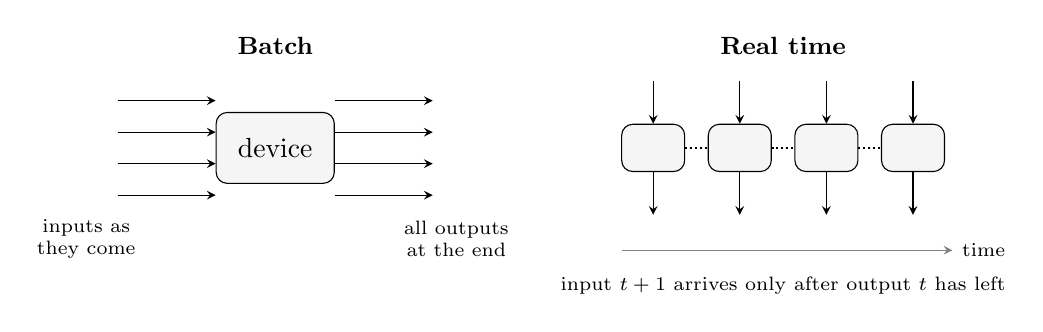
\begin{tikzpicture}[>=stealth, box/.style={draw, rounded corners, minimum width=1.5cm, minimum height=0.9cm, fill=gray!8}]
  \node[font=\small\bfseries] at (2.6,1.6) {Batch};
  \node[box] (B) at (2.6,0.3) {device};
  \foreach \i/\y in {1/0.9,2/0.5,3/0.1,4/-0.3} {\draw[->] (0.6,\y) -- (B.west |- 0,\y);}
  \foreach \i/\y in {1/0.9,2/0.5,3/0.1,4/-0.3} {\draw[->] (B.east |- 0,\y) -- (4.6,\y);}
  \node[font=\scriptsize, align=center] at (0.2,-0.85) {inputs as\\they come};
  \node[font=\scriptsize, align=center] at (4.9,-0.85) {all outputs\\at the end};
  \begin{scope}[xshift=7cm]
  \node[font=\small\bfseries] at (2.05,1.6) {Real time};
  \foreach \t in {0,1,2,3} {
    \node[box, minimum width=0.8cm, minimum height=0.6cm] (D\t) at (1.1*\t+0.4,0.3) {};
    \draw[->] (1.1*\t+0.4,1.15) -- (D\t.north);
    \draw[->] (D\t.south) -- (1.1*\t+0.4,-0.55);
  }
  \foreach \t in {0,1,2} {\draw[densely dotted, thick] (1.1*\t+0.8,0.3) -- (1.1*\t+1.1,0.3);}
  \draw[->, gray] (0,-1.0) -- (4.2,-1.0) node[right, font=\scriptsize, black] {time};
  \node[font=\scriptsize, align=center] at (2.05,-1.45) {input $t+1$ arrives only after output $t$ has left};
  \end{scope}
\end{tikzpicture}
\caption{A batch device may hold its outputs until the end. A real-time device releases each output before the next input arrives; it may carry any memory forward (dotted), but it cannot hold an output back.}
\label{fig:devices}
\end{figure}

For agents that give classical answers to classical questions, with answers that depend on past ones, Thompson, Riechers, Garner, Elliott and Gu asked this question and called the answer the work cost of online response: the extra work needed to emit each output before the next input, compared with answering in long blocks~\cite{Thompson25}. That cost comes from the memory such a strategy needs, and a quantum memory can reduce it. We ask the question for channels, which need no memory, with quantum inputs and outputs. For devices built from energy-conserving dynamics and heat baths, the answer is yes, but only for quantum channels, and we find the exact price. Throughout, the device applies the same channel again and again, and the task itself needs no memory between uses; when later steps of a process depend on earlier inputs whose outputs have already left, timing costs appear even for classical processes (Section~\ref{sec:discussion}). We take the free operations to be thermal operations. If every Gibbs-preserving map were free, every Gibbs-preserving channel could be applied round by round at no cost, and the question would take a different form.

Write $H$ for the Hamiltonian and $\beta=1/\kB T$, and measure work in units of $\kB T\ln2$. For a time-covariant channel, the batch cost is a maximum over inputs $\rho$ of an entropy cost and an energy cost,
\begin{equation}\label{eq:batch}
  \Tcap(\Phi)=\max_\rho\Bigl[S(\rho)-S(\Phi(\rho))+\tfrac{\beta}{\ln 2}\Tr H\bigl(\Phi(\rho)-\rho\bigr)\Bigr],
\end{equation}
in bits; Faist, Berta and Brand\~ao use nats. The entropy that the process removes from the system has to go somewhere, and the energy it adds has to come from somewhere. We show that the real-time cost has the same form,
\begin{equation}\label{eq:realtime}
  \Trt(\Phi)=\sup_{\rho>0}\Bigl[s_\rho(\Phi)+\tfrac{\beta}{\ln 2}\Tr H\bigl(\Phi(\rho)-\rho\bigr)\Bigr],
\end{equation}
with one change. The entropy cost $S(\rho)-S(\Phi(\rho))$ is replaced by the \emph{real-time entropy cost} $s_\rho(\Phi)$: the least entropy that one use on input $\rho$ must leave behind in a device that held no information about that input beforehand (Definition~\ref{def:rtcost}). Equivalently,
\begin{equation}\label{eq:mutual}
  s_\rho(\Phi)=S(\rho)-S(\Phi(\rho))+m_\rho(\Phi),
\end{equation}
where $m_\rho(\Phi)\ge0$ is the least mutual information that an implementation of $\Phi$ must leave between the output and what stays behind in the device (Section~\ref{sec:setting}). So $\Trt\ge\Tcap$. For time-covariant channels the difference is the price of real time; for other channels, a device whose clock must return can pay more than $\Tcap$ even in batch~\cite{KeepingTime}. We call $\Trt(\Phi)$ the \emph{real-time work rate}.

The extra term has a simple source. A process leaves entropy in its bath, correlated with its output. The batch device of Faist, Berta and Brand\~ao removes that correlation by erasing the environments with the outputs as side information, up to an error that can be made arbitrarily small for large $n$~\cite[Thm.~7.1]{FBB21}; the conditioning in~\cite{FDOR15} has the same origin. A real-time device has already released its outputs, so it cannot use them to recover this correlation. The term $m_\rho$ is a cost at a fixed input. The surcharge between the optimal rates of a time-covariant channel, the difference between the maxima in~\eqref{eq:realtime} and~\eqref{eq:batch}, is generally neither the largest $m_\rho$ nor $m_\rho$ at either optimal input, because the two maxima can sit at different inputs: for amplitude damping at $p=1/2$ and $\beta\Delta=\ln2$ the surcharge is $0.431$ bits per use, while $m_\rho$ is $0.918$ bits at the real-time optimum and $0.197$ bits at the batch optimum~\cite{TimeOrder}.

Partial reset shows the mechanism. Let a qubit with energy gap $\Delta$ decay to its ground state with probability $p$. The natural dilation sends $|1\rangle|0\rangle_E$ to $\sqrt{1-p}\,|1\rangle|0\rangle_E+\sqrt p\,|0\rangle|1\rangle_E$, so for $0<p<1$ the output stays entangled with the environment, which records whether the decay happened. A batch device can erase that record later, using the output it still holds; a real-time device has released the output and cannot, and no other implementation avoids the correlation (Theorem~\ref{thm:classical}). For full reset, $p=1$, the output is always the ground state, nothing is correlated with it, and timing costs nothing.

\paragraph{The model in brief.} Work is counted over a full cycle. Heat baths start in thermal states, all dynamics conserve energy, the device's controller returns to its initial state, and a battery supplies the difference. Outputs leave one at a time and are never touched again, and the error is measured against the most demanding observer, who may choose inputs adaptively and keep quantum references. Table~\ref{tab:contract} collects the contract, and Section~\ref{sec:setting} states it in full.

\begin{table}[t]
\centering
\small
\begin{tabular}{@{}>{\raggedright\arraybackslash}p{2.6cm}>{\raggedright\arraybackslash}p{12.2cm}@{}}
\toprule
Part of the contract & What it requires\\
\midrule
Target & $n$ uses of one channel $\Phi$ on a system with Hamiltonian $H$, time-covariant in Theorems~\ref{thm:law}--\ref{thm:werner}.\\
Access & Real time: input $t+1$ is supplied only after output $t$ has left, and a released output is never touched again. Batch: all outputs may be held until the end.\\
Observer and error & The observer chooses inputs adaptively and keeps quantum references. The error is the largest trace distance over all such observers between the actual and the ideal interaction; in batch, the half diamond distance to $\Phi^{\otimes n}$.\\
Free dynamics & Unitaries that commute with the total Hamiltonian of the systems they act on, and reservoir cells declared in advance that start in Gibbs states, independent of each other and of everything else. Measurements and records are counted; there is no external coherence and no Gibbs-preserving map supplied as a black box.\\
Controller & Holds all hardware, including memory and clocks. It returns exactly in the constructions for time-covariant channels and approximately in Theorem~\ref{thm:clock}; the lower bounds need only that its free energy returns up to $o(n)$. In the fixed-error converse it starts in a thermal state.\\
Battery & Mechanical: work is its mean loss of energy, and its entropy changes by $o(n)$. Deterministic work: it starts in an energy eigenstate and ends in a fixed one with probability tending to one, with mean energy within $o(n)$ of it. A stationary battery holds no phase reference.\\
Limit & The rate is per use, as $n\to\infty$ with error tending to zero. Reservoirs, controllers and running times may have any finite size. At zero error the batch saving can disappear (Proposition~\ref{prop:extreme}).\\
\bottomrule
\end{tabular}
\caption{The operational contract. Section~\ref{sec:setting} states it in full; individual theorems add or relax conditions where they say so.}\label{tab:contract}
\end{table}

\paragraph{Main results.} Theorems~\ref{thm:law}--\ref{thm:werner} concern time-covariant channels: those that commute with the time evolution generated by $H$, which are the ones energy-conserving dynamics can implement without an external clock~\cite{Lostaglio15,FBB21}.

\begin{theorem}[Real-time work law]\label{thm:law}
Let $\Phi$ be time-covariant. In real time, the optimal work per use at vanishing error is $\kB T\ln 2\,\Trt(\Phi)$. Moreover, for every fixed $\delta>0$, any implementation whose controller starts in a thermal state and that draws at most $n\kB T\ln 2\,(\Trt(\Phi)-\delta)$ of deterministic work, meaning that its battery ends in a definite energy level with probability tending to one, has error tending to one as $n\to\infty$.
\end{theorem}

At zero Hamiltonian the first statement, in purity units, is in our earlier work~\cite{Memory,ImmediateDelivery,ClosedMemory}, and so is the second at zero rate~\cite{Flagship}. In batch, the converse of Faist, Berta and Brand\~ao already holds at every fixed error below $1/2$~\cite[Prop.~4.2]{FBB21}.

The rate is a maximum over inputs of a minimum over implementations, while a device is built once and must serve every input and every observer. Part of Theorem~\ref{thm:law} is that the two orders agree: one device costs no more per use than the hardest input, as Faist, Berta and Brand\~ao found in batch for time-covariant channels~\cite{FBB19}. For this real-time functional the interchange holds for every channel (Lemma~\ref{lem:minimax}); time covariance lets the construction of Theorem~\ref{thm:law} attain it with a controller that returns exactly, and Theorem~\ref{thm:clock} attains it for every channel with one that returns approximately. In batch with a returned clock, the analogous interchange between choosing a device and choosing an input can fail. For example, $X$-dephasing on a qubit with energy gap $\Delta$ costs $\Delta/2$ per use for any device that is correct on every input~\cite{KeepingTime}, while each known input can be served at no more than the thermodynamic capacity, by the fixed-input construction of Faist, Berta and Brand\~ao, whose coherent source is small enough to be returned~\cite[Prop.~8.3]{FBB21},~\cite{KeepingTime}.

The two costs differ in a single term. It vanishes for classical channels, but not for a partial quantum reset.

\begin{theorem}[Classical channels pay no surcharge; partial reset does]\label{thm:classical}\leavevmode
\begin{enumerate}[label=(\alph*), leftmargin=*]
\item If $\Phi$ is classical, meaning that it measures in an eigenbasis of $H$ and prepares states diagonal in that basis, then $\Trt(\Phi)=\Tcap(\Phi)$ at every temperature.
\item Let $\Phi$ be amplitude damping with probability $p$ on a qubit with energy gap $\Delta$. Then $\Trt(\Phi)=\max_{0\le y\le p}\bigl[h(y)-\beta\Delta y/\ln 2\bigr]$, where $h$ is the binary entropy. For $0<p<1$, $\Trt(\Phi)>\Tcap(\Phi)$ at every temperature. For $p=1$, $\Trt(\Phi)=\Tcap(\Phi)$.
\end{enumerate}
\end{theorem}

Amplitude damping with $p=1$ is a full reset to the ground state, the process of Landauer's principle, and timing does not change its cost. Partial reset is different. Its output stays correlated with what the process leaves behind, and in real time that correlation costs work at every temperature (Figure~\ref{fig:damping}).

The surcharge can be as large as the whole cost. For exact implementations we count the free energy $w$ drawn from the battery and the controller (Section~\ref{sec:law}); with a mechanical battery whose entropy changes by $o(n)$ and a controller that returns, this is the work up to $o(n)$.

\begin{theorem}[Werner--Holevo]\label{thm:werner}
Let $W(\rho)=(\Tr(\rho)\,I-\rho^{T})/2$ be the Werner--Holevo channel on a qutrit with zero Hamiltonian. The free energy $w$, in bits, needed for $n$ uses satisfies
\begin{center}
\begin{tabular}{lcc}
\toprule
 & exact & error $n^{-2}$\\
\midrule
real time & $w\ge n\log_23$ & $w\ge n\log_23-O(\log n)$\\
batch & $w\ge n\log_23$ & $w=O(\log n)$ achievable\\
\bottomrule
\end{tabular}
\end{center}
Both exact bounds are attained with an information battery, and the real-time work rate is $\Trt(W)=\log_23$.
\end{theorem}

In purity units these statements are in our earlier work~\cite{ImmediateDelivery}, and the batch rate of zero follows from the theorem of Faist, Berta and Brand\~ao. Here they are statements about free energy. The batch saving comes from tolerating a vanishing error, not from an exact refund.

\paragraph{Further results.} Four further results complete the picture. At zero error the saving of waiting disappears for every extreme channel, such as Werner--Holevo and amplitude damping with $0<p<1$: a batch device then pays the full real-time rate (Proposition~\ref{prop:extreme}, Section~\ref{sec:werner}). In real time a channel costs nothing exactly when it is a limit of thermal operations (Theorem~\ref{thm:free}, Section~\ref{sec:free}); this is a robust, work-cost form of the criterion of Lie et al.~\cite{LieEtAl26}, and it identifies the processes that are free in batch but cost work in real time. A device whose clock must return exactly, and whose battery holds no phase reference, cannot run a channel that is not time-covariant, whatever work is spent (Proposition~\ref{prop:clock}), while a clock that may return approximately runs every channel at the rate $\Trt$ (Theorem~\ref{thm:clock}, Section~\ref{sec:free}). Finally, whether a generalized dephasing channel is free in real time is undecidable in a fixed dimension (Theorem~\ref{thm:undecidable}, Section~\ref{sec:undecidable}).

\paragraph{Relation to prior work.} The batch cost is the thermodynamic capacity of Faist, Berta and Brand\~ao~\cite{FBB19,FBB21}, which had appeared as the work value of channel uses~\cite{NGP15}. Their converse rests on single-shot work costs for a fixed input: the smooth max-entropy of the discarded information conditioned on the output, for degenerate Hamiltonians~\cite{FDOR15}, and the coherent relative entropy in general~\cite{FR18}. The last step of their thermal-operation construction, erasing the environments with the outputs as side information, a universal form of the conditional erasure of~\cite{delRio11} built by position-based decoding~\cite[Sec.~7]{FBB21}, is the step a real-time device cannot take. They suggested replacing the diamond norm by distinguishability measures for processes with memory~\cite{Chiribella08}, noting that this ``would be particularly relevant for settings with memory effects, for instance implementations of gates in a quantum computer''~\cite{FBB19}. Our real-time error is a measure of this kind~\cite{Chiribella08,GutoskiWatrous07}.

Ryb\'ar and Ziman introduced repeatable channels, implemented again and again by one device with a finite memory and no resets, so that every use acts as the same channel. They showed that every mixture of unitaries is repeatable and that no non-unital channel is, because the memory must absorb $S(\rho)-S(\Phi(\rho))$ of entropy per use~\cite{RybarZiman}; Lemma~\ref{lem:accumulation} is the conditional form of their entropy count. Whether a unital channel that is not a mixture of unitaries can be repeatable they left open; the Werner--Holevo channel cannot, since every exact round adds $\log_23$ bits to the device (Theorem~\ref{thm:werner}). Work extraction under causal constraints has been studied for multitime processes~\cite{ZambonAdesso}, for temporally correlated sequences of states~\cite{HuangTOFE} and for agents that act on environments with memory~\cite{Fiderer26}; the online execution of classical strategies with memory has a work cost of its own, which quantum memory can reduce~\cite{Thompson25}. Here we price the implementation of a memoryless channel with quantum inputs and outputs instead.

Quantum processes are known to dissipate more than classical ones with non-orthogonal inputs or compressed memories~\cite{BedinghamMaroney,LoomisCrutchfield20,RiechersGu21}; here the excess comes from timing alone. Classical processes can incur online costs under other constraints, such as a fixed protocol, a modular design or periodic operation~\cite{KolchinskyWolpert21,BMC18,OuldridgeWolpert23}. Our devices may carry any memory and act jointly on everything they hold, so these constraints are absent; the real-time surcharge is instead a modularity cost in time, since the device can no longer act on the outputs it has released (Section~\ref{sec:discussion}).

Our earlier work proves the zero-Hamiltonian, purity-unit forms of the rate statement in Theorem~\ref{thm:law}, of Theorem~\ref{thm:werner} and of Theorem~\ref{thm:free}~\cite{Memory,ImmediateDelivery,ClosedMemory}, a strong converse at zero rate, and undecidability for dephasing channels of unbounded dimension~\cite{Flagship}. New here are the finite-temperature law with work in place of purity, the converse at every fixed error and every rate below $\Trt$, Theorem~\ref{thm:classical}, the robust finite-temperature form of Theorem~\ref{thm:free}, Theorem~\ref{thm:clock}, and the fixed-dimension and non-enumerability statements of Theorem~\ref{thm:undecidable}.

\paragraph{Outline.} Section~\ref{sec:setting} sets up the model. Section~\ref{sec:law} proves Theorem~\ref{thm:law}. Section~\ref{sec:classical} treats classical channels and reset, Section~\ref{sec:werner} the Werner--Holevo channel, Section~\ref{sec:free} what is free and what a clock can do, and Section~\ref{sec:undecidable} undecidability. Section~\ref{sec:discussion} discusses an experimental test and open problems. The longer constructions are in the appendices. A companion paper~\cite{TimeOrder} places this law among general schedules of arrivals, releases and loans.


\section{Setting}\label{sec:setting}

Fix a $d$-level system $A$ with Hamiltonian $H$, an inverse temperature $\beta=1/\kB T>0$, and the Gibbs state $\gamma=e^{-\beta H}/\Tr e^{-\beta H}$. Entropies and logarithms are base two. A channel $\Phi$ on $A$ is \emph{time-covariant} if $\Phi(e^{-iHt}\rho\, e^{iHt})=e^{-iHt}\Phi(\rho)e^{iHt}$ for all $t$. Energy-conserving dynamics without an external phase reference can only implement such channels~\cite{Lostaglio15,FBB21}.

\paragraph{The device.} An implementation consists of a controller $C$, a battery $B$ and a reservoir $R$. The controller holds all hardware: memory, clocks, catalysts and any work registers not charged to the battery. The reservoir is a finite collection of cells, each with its own Hamiltonian. All cells are declared in advance, including those used only late or only after the last output. They start in their Gibbs states at inverse temperature $\beta$, independent of each other and of everything else. The initial state is $\alpha_C\otimes\zeta_B\otimes\gamma_R$, with an additive Hamiltonian $H_C+H_B+H_R$. Every operation is a unitary that commutes with the total Hamiltonian of the systems it acts on. Measurements and records are part of the dilation and are counted. No other resource is free: there is no external coherence, no Gibbs-preserving map supplied as a black box, and no initial correlation between $C$, $B$ and $R$. The battery is \emph{stationary} if $\zeta_B$ commutes with $H_B$, as an energy eigenstate does. A stationary battery holds no phase reference, so every clock of the device is then in its controller.

\paragraph{Real-time operation.} The device serves $n$ rounds. In round $t$ an input system arrives, the device acts on it together with its internal systems, and the output is released. Input $t+1$ is supplied only after output $t$ has left. Between rounds, and after the last one, the device may act on its internal systems as it likes. It never acts again on a delivered output. The inputs come from an observer who may choose them adaptively and keep quantum references. The \emph{error} $\varepsilon$ is the largest trace distance $\tfrac12\|\cdot\|_1$, over all such observers, between the final state of the observer's systems with the device and with $n$ ideal uses of $\Phi$. This is the distance between strategies of~\cite{Chiribella08,GutoskiWatrous07}.

\paragraph{Batch operation.} For comparison, a batch implementation may hold all outputs until the end. Its error is the half diamond distance to $\Phi^{\otimes n}$, the criterion of~\cite{FBB21}.

\paragraph{Work.} The controller must return. For the constructions of time-covariant channels it returns exactly to $\alpha_C$, independent of all other systems, and Theorem~\ref{thm:clock} relaxes this for the other channels; for the lower bounds it is enough that its free energy returns up to $o(n)$. The battery is mechanical: work is its mean loss of energy, and its entropy changes by $o(n)$, so it cannot hide a second bath. Work is \emph{deterministic} when the battery starts in an energy eigenstate, ends, with probability tending to one for every observer, in a fixed energy eigenstate, and its mean energy differs from that eigenvalue by $o(n)$ (a signed mean deviation; some statements in the companion papers use the stronger mean absolute deviation $\Tr|H_B-E|\rho_B$, and say so); this is the mechanical counterpart of the information battery checked by a projector in~\cite{FR18,FBB21}. The last clause matters only for a controller that returns approximately (Section~\ref{sec:free}): it prevents a broad reference from lending the device energy that the battery repays in one rare, large event. In the fixed-error statement of Theorem~\ref{thm:law} the controller also starts in a thermal state (Remark~\ref{rem:thermal-controller}). For a family of implementations with error $\varepsilon_n\to0$, the \emph{work rate} is $\limsup_n W_n/(n\kB T\ln 2)$, in bits per use. The optimal real-time and batch rates are the infima over such families.

These rates allow reservoirs, controllers and running times of any finite size. They describe what is possible in principle, not an efficient or autonomous engine.

\begin{remark}[Battery models]
Faist, Berta and Brand\~ao count work as purity in an information battery~\cite{FR18,FBB21}; we use a mechanical battery, so that work is energy. Our lower bounds are statements about the free energy drawn from battery and controller (Lemma~\ref{lem:accounting}), so they hold in both conventions. We quote $\Tcap$ as the batch benchmark in their convention.
\end{remark}

\begin{definition}[Real-time entropy cost]\label{def:rtcost}
Let $\psi_\rho$ purify a full-rank input $\rho$ with reference $Q$, and let $\chi_\rho=(\mathrm{id}_Q\otimes\Phi)(\psi_\rho)$ on $QO$. For $\varepsilon>0$ let
\[
s_{\rho,\varepsilon}(\Phi)=\inf S(QO|F)_\sigma,
\]
over finite systems $F$ and states $\sigma_{QOF}$ with $\sigma_{QF}=\rho^{T}\otimes\sigma_F$ and $\tfrac12\|\sigma_{QO}-\chi_\rho\|_1\le\varepsilon$. The \emph{real-time entropy cost} is $s_\rho(\Phi)=\lim_{\varepsilon\downarrow0}s_{\rho,\varepsilon}(\Phi)$.
\end{definition}

Think of $F$ as a purification of everything the device holds when the input arrives. The product condition $\sigma_{QF}=\rho^T\otimes\sigma_F$ says that none of it carries information about the fresh input. After the round, $S(QO|F)$ equals the increase in the entropy of the device's internal state (Lemma~\ref{lem:accumulation}). So $s_\rho(\Phi)$ is the least entropy that one use on input $\rho$ must add to a device that did not know the input in advance. Since $S(QO|F)\ge S(Q)-S(O)$ whenever $QF$ is a product, $s_\rho(\Phi)\ge S(\rho)-S(\Phi(\rho))$. At zero Hamiltonian, $\Trt(\Phi)=\sup_\rho s_\rho(\Phi)$ is the purity cost of real-time operation of our earlier work, where it is written $\kappa(\Phi)$~\cite{Memory,ImmediateDelivery,ClosedMemory}.

There is a second way to read $s_\rho$. A dilation of $\Phi$ is a unitary $U$ on the input and a bath in state $\tau$ with $\Phi(\rho)=\Tr_E U(\rho\otimes\tau)U^*$. On input $\rho$ it ends with the output $O$ and the bath $E'$ in a joint state, and conservation of entropy gives $S(E')-S(\tau)=S(\rho)-S(\Phi(\rho))+I(O{:}E')$. The real-time entropy cost is the infimum of $S(E')-S(\tau)$ over exact finite dilations, input by input~\cite{ClosedMemory}. Hence~\eqref{eq:mutual} holds with
\[
m_\rho(\Phi)=\inf\bigl\{\,I(O{:}E')_\rho:\ (U,\tau)\ \text{a finite dilation of}\ \Phi\,\bigr\}.
\]
The batch cost is the same expression with $m_\rho=0$. A batch device approaches it by erasing its baths with the outputs as side information~\cite[Sec.~7]{FBB21}. This works up to an error that can be made arbitrarily small for large $n$; at zero error it can fail completely (Theorem~\ref{thm:werner}).

\section{The real-time work law}\label{sec:law}

The lower bound comes from two facts: a bookkeeping identity that holds for every implementation, and a bound on how much entropy each real-time round must add to the device. The upper bound is a construction. Section~\ref{sec:fixed-error} upgrades the lower bound to every fixed error.

\subsection{Bookkeeping}

Write $D=CBR$ for everything except the inputs and outputs, and let $A=S(D_{\mathrm{fin}})-S(D_{\mathrm{init}})$ be the entropy it gains. Let $\Delta E_{\mathrm{sys}}$ be the total energy delivered in the outputs minus the total energy taken from the inputs. Measure the free energy drawn from the battery and the controller in units of $\kB T\ln2$:
\[
w=\frac{F(\zeta_{\mathrm{init}})-F(\zeta_{\mathrm{fin}})+F(\alpha_{\mathrm{init}})-F(\alpha_{\mathrm{fin}})}{\kB T\ln 2},\qquad F(x)=\Tr(H x)-\kB T\ln2\,S(x).
\]

\begin{lemma}[Accounting identity]\label{lem:accounting}
For every implementation in the model of Section~\ref{sec:setting},
\[
w=A+\tfrac{\beta}{\ln2}\,\Delta E_{\mathrm{sys}}+D(R_{\mathrm{fin}}\|\gamma_R)+I(C{:}B{:}R)_{\mathrm{fin}},
\]
where $I(C{:}B{:}R)=S(C)+S(B)+S(R)-S(CBR)$ is the total correlation. In particular $w\ge A+\beta\Delta E_{\mathrm{sys}}/\ln2$.
\end{lemma}

\begin{proof}
Energy conservation gives $\Delta E_C+\Delta E_B+\Delta E_R+\Delta E_{\mathrm{sys}}=0$. For the reservoir, $S(R_{\mathrm{fin}})-S(\gamma_R)=\beta\Delta E_R/\ln2-D(R_{\mathrm{fin}}\|\gamma_R)$. Since $C$, $B$ and $R$ start independent, $A=\Delta S_C+\Delta S_B+\Delta S_R-I(C{:}B{:}R)_{\mathrm{fin}}$. Substituting into $w=\Delta S_B+\Delta S_C-\beta(\Delta E_B+\Delta E_C)/\ln2$ gives the identity.
\end{proof}

This is multipartite finite-reservoir Landauer bookkeeping~\cite{ReebWolf14}. Correlations with the observer do not enter, because the identity concerns only the device. A reservoir cell that is set aside can be kept in $R$ and left alone, so discarding never helps. Correlations that the controller keeps with past outputs, and catalysts it returns at the end, only add to $w$ through the last two terms.

\subsection{What each round must leave behind}

\begin{lemma}[Causal accumulation]\label{lem:accumulation}
Suppose the error is at most $\varepsilon$, and the observer feeds each round one half of a fresh purification $\psi_\rho$ of a full-rank state $\rho$, keeping all references. Then in every round the entropy of the device rises by at least $s_{\rho,\varepsilon}(\Phi)$, so $A\ge n\,s_{\rho,\varepsilon}(\Phi)$.
\end{lemma}

\begin{proof}
Let $D_t$ be the device before round $t$ and let $F_t$ purify it; $F_t$ contains the earlier references and outputs. The fresh pair $Q_tS_t$ is independent of $D_tF_t$, and the round acts on $S_tD_t$ only, so $Q_tF_t$ stays a product. After the round the global state is pure, which gives $S(D_{t+1})-S(D_t)=S(Q_tO_t|F_t)$. The observer's state $Q_tO_t$ is within $\varepsilon$ of $\chi_\rho$, so this extension is feasible in Definition~\ref{def:rtcost} and $S(Q_tO_t|F_t)\ge s_{\rho,\varepsilon}(\Phi)$. Operations on the device between rounds are unitary on $D$ and preserve its entropy, so the increments add up.
\end{proof}

The device's memory may be correlated with every earlier output; the lemma allows that. What it rules out is a memory that already knows the next input.

\subsection{The lower bound}

Each delivered output is within $\varepsilon$ of $\Phi(\rho)$, so its energy is within $\varepsilon\,\mathrm{span}(H)$ of $\Tr H\Phi(\rho)$, where $\mathrm{span}(H)$ is the difference between the largest and smallest eigenvalues. Combining the two lemmas with the same input $\rho$,
\begin{equation}\label{eq:converse}
w\ \ge\ n\Bigl[s_{\rho,\varepsilon}(\Phi)+\tfrac{\beta}{\ln2}\Tr H\bigl(\Phi(\rho)-\rho\bigr)-\tfrac{\beta\varepsilon}{\ln2}\,\mathrm{span}(H)\Bigr]
\end{equation}
for every full-rank $\rho$. For a mechanical battery the actual work is $\kB T\ln2\,(w-\Delta S_B)$ when the controller returns, and $\Delta S_B=o(n)$. Letting $\varepsilon\to0$ and taking the supremum over $\rho$ gives the lower half of Theorem~\ref{thm:law}. Neither time covariance nor a known horizon is used: the lower bound holds for every channel, and for any controller, including one that carries a phase reference. Recovery after the last output does not help either, since every reservoir cell used for it is already part of $D$.

\subsection{The construction}

The matching construction has three layers (Appendix~\ref{app:construction}).

\emph{A real-time dilation.} For every $\eta>0$ there is a finite dilation of $\Phi$, a unitary $U$ acting on the input and a bath in state $\tau$, whose cost $\sup_\rho[S(\text{bath output})-S(\tau)+\beta\Tr H(\Phi(\rho)-\rho)/\ln2]$ is within $\eta$ of $\Trt(\Phi)$. This uses the identity $\lim_{\varepsilon\to0}s_{\rho,\varepsilon}=\inf_{\text{exact dilations}}[S(\text{bath output})-S(\tau)]$, input by input~\cite{ClosedMemory}, together with a minimax argument; the energy term is the same for every exact dilation.

\emph{Paying for entropy and energy together.} Running the dilation $n$ times, with a fresh bath copy each round, leaves the used baths in a state supported, up to exponentially small weight, on a subspace whose Gibbs weight is controlled by $\Trt(\Phi)+\eta$ bits per round. A single energy register records the total energy exchanged with the system. A positive-operator inequality, which survives arbitrary correlations between the baths, the register, the references and adaptively chosen inputs, charges entropy and energy on the same input. This plays the role of the universal conditional and relative typical operator of Faist, Berta and Brand\~ao, which also counts entropy against energy and serves every input type at once~\cite{FBB19}, \cite[Sec.~6]{FBB21}; here the universality comes instead from a single dilation chosen by the minimax argument and one operator inequality. Time covariance is used here: it lets an energy-conserving lift of $U$ reproduce the whole adaptive experiment exactly.

\emph{Paying the work.} An energy-conserving converter between two subspaces of given Gibbs weight moves a battery by the logarithm of their ratio, with any sign. It is built from reservoirs with integer degeneracies and exact energy-conserving swaps, and it preserves coherences. The device forms its fresh baths at the start, keeps every used bath until the last output has left, and then converts the used baths back. It never touches a delivered output. The net debit is $n\kB T\ln2\,(\Trt(\Phi)+\eta)+o(n)$, and a final swap with a thermal cell returns the controller exactly. This refund cannot recover the correlations between the used baths and the outputs, because the outputs are gone; those correlations are what the batch construction of~\cite[Sec.~7]{FBB21} recovers, asymptotically, by erasing the baths with the outputs as side information.

\begin{remark}[Known horizon]
The construction assumes that $n$ is known in advance, as does the zero-Hamiltonian purity law~\cite{ClosedMemory}. We expect a schedule of growing blocks to reach the same rate without this assumption, with supplies brought in as needed and a final clean-up, but we do not prove it here.
\end{remark}

\begin{remark}[Batch]
Faist, Berta and Brand\~ao implement $\Phi^{\otimes n}$ with thermal operations at work rate $\Tcap(\Phi)$ for time-covariant $\Phi$, counting work in an information battery, and no batch implementation does better~\cite[Thm.~7.1, Prop.~4.2]{FBB21}. In our model the batch lower bound is $w\ge n[S(\rho)-S(\Phi(\rho))+\beta\Tr H(\Phi(\rho)-\rho)/\ln2]-\varepsilon n\log d-h(\varepsilon)$ up to the same energy correction, by subadditivity and continuity of entropy on the $n$ outputs.
\end{remark}

\subsection{Every fixed error}\label{sec:fixed-error}

The lower bound~\eqref{eq:converse} is a rate statement: it says nothing about an implementation that accepts a fixed error $\varepsilon=0.1$, say. In batch, the converse of Faist, Berta and Brand\~ao already holds at every fixed error below $1/2$~\cite[Prop.~4.2]{FBB21}. In real time, the following theorem covers every error below one, provided the work is deterministic.

\begin{theorem}[Fixed-error converse]\label{thm:fixed-error}
Let $\Phi$ be time-covariant and $\delta>0$. There are constants $a,b,c>0$, depending only on $\Phi$, $H$, $\beta$ and $\delta$, with the following property. Consider any real-time implementation whose controller and reservoirs start thermal and independent, and whose battery starts in a pure energy eigenstate of energy $E_{\mathrm{init}}$. Let $P$ be a projector onto battery eigenstates whose Gibbs weight $\Tr Pe^{-\beta H_B}$ is at most $2^{n(\Trt(\Phi)-\delta)}e^{-\beta E_{\mathrm{init}}}$, and let $q$ be the largest probability, over observers, that the battery ends outside $P$; it suffices to take the observer of Appendix~\ref{app:fixed-error}. Then
\[
1-\varepsilon_n\ \le\ q+c\,e^{-bn}+2^{-an}.
\]
\end{theorem}

For a battery that ends in a single eigenstate of energy $E_{\mathrm{fin}}$, the Gibbs-weight condition says exactly that the work $E_{\mathrm{init}}-E_{\mathrm{fin}}$ is at most $n\kB T\ln2\,(\Trt(\Phi)-\delta)$. So with deterministic work below the real-time rate, the error tends to one, exponentially fast if the battery never misses its target.

The proof (Appendix~\ref{app:fixed-error}) tests a random fraction of the rounds with an energy-conserving measurement, so that entropy accumulation~\cite{DFR20} applies, and caps the probability of passing by a smooth min-entropy bound weighted by Gibbs factors. The weighting is what makes the argument work at finite temperature: the reservoir's partition function cancels exactly, whatever the size of the reservoir.

\begin{remark}[Mean work is not enough]
Deterministic work cannot be replaced by mean work. Toss a thermal coin: with probability $1-\varepsilon$ run an optimal implementation, and otherwise run a free channel. The error is at most $\varepsilon$, the battery entropy at most one bit, and the mean work is $(1-\varepsilon)$ times the optimum. At fixed error, mean work can therefore fall below the real-time rate by a constant fraction.
\end{remark}

\begin{remark}[Why the controller must start thermal]\label{rem:thermal-controller}
The thermal start of the controller cannot simply be dropped. A controller that only returns approximately can carry an incoherent energy bank whose loans depend on the branch and cancel in the mean; with it a covariant reset runs at half the vanishing-error rate with error exactly $1/2$~\cite{KeepingTime}, although the battery's debit is the same on every branch. What decides this is how spread out the controller's capital is, not its size. A spread $o(n/\sqrt\eta)$, where $\eta$ is the controller's return error, still forces a strong converse, but only at the thermodynamic capacity, which can lie below $\Trt$; a bank of spread of order $n/\sqrt\eta$ can break even that~\cite{KeepingTime}. Whether the converse at $\Trt$ survives such a controller is open.
\end{remark}

\section{Classical channels and reset}\label{sec:classical}

We first record a tool that settles the real-time entropy cost whenever the environment of a channel determines its input. Let $V:A\to O\otimes E$ be a Stinespring isometry of $\Phi$ and $\Phi^c(\rho)=\Tr_O V\rho V^*$ its complementary channel.

\begin{lemma}[Invertible environment]\label{lem:invertible}
If $\Phi^c$ is invertible as a linear map, then $s_\rho(\Phi)=S(\Phi^c(\rho))$ for every full-rank $\rho$.
\end{lemma}

\begin{proof}[Proof idea]
Take an exact extension $\sigma_{QOF}$, with $\sigma_{QO}=\chi_\rho$ and $\sigma_{QF}=\rho^T\otimes\sigma_F$. By uniqueness of purification, $\sigma_{QOF}=(\mathrm{id}_{QO}\otimes\Lambda)(\psi_{QOE})$ for a channel $\Lambda:E\to F$, where $\psi_{QOE}$ is the purification of $\chi_\rho$ given by $V$. The product condition says that $\Lambda\circ\Phi^c$ sends every input to $\sigma_F$. Since $\Phi^c$ is invertible, $\Lambda$ itself is constant, so $\sigma_{QOF}=\chi_\rho\otimes\sigma_F$ and $S(QO|F)=S(\chi_\rho)=S(\Phi^c(\rho))$. The extension $\chi_\rho\otimes\sigma_F$ is always feasible, so this is the exact value. For approximate extensions, Uhlmann's theorem and the bounded inverse give the same limit, with estimates that do not depend on the size of $F$ (Appendix~\ref{app:invertible}).
\end{proof}

So when the environment determines the input, the best a real-time device can do is the plain Stinespring dilation: keep the environment and pay its entropy.

\subsection{Classical channels}

Let $\Phi$ measure in an eigenbasis $\{|i\rangle\}$ of $H$ and prepare a diagonal state, $\Phi(\rho)=\sum_{i,j}P(j|i)\langle i|\rho|i\rangle\,|j\rangle\langle j|$ for a stochastic matrix $P$.

\begin{proof}[Proof of Theorem~\ref{thm:classical}(a)]
Two facts about classical channels carry the proof (Appendix~\ref{app:classical}). First, on a diagonal input $p$ the real-time entropy cost equals the batch one, $s_p(\Phi)=H(p)-H(Pp)$. The device writes the output as an exact function $Y=f(X,R)$ of the input and a finite random seed $R$. It then hides the seed in a bath whose spectrum is close to log-uniform, so that the bath ends almost independent of the output. Second, coherent inputs do no better than their diagonal parts: a random phase applied from a flat register removes the coherence at no cost, so $s_\rho(\Phi)\le H(\mathrm{diag}\,\rho)-H(P\,\mathrm{diag}\,\rho)$. The energy term depends only on the populations of $\rho$ and $\Phi(\rho)$. Hence the supremum in~\eqref{eq:realtime} may be taken over diagonal inputs, where it coincides with the maximum in~\eqref{eq:batch} restricted to diagonal inputs. That is at most $\Tcap(\Phi)$, and $\Trt\ge\Tcap$ always.
\end{proof}

The construction keeps a record of the input and erases it against a bath, an idea that goes back to Bennett~\cite{Bennett73}. What the proof adds is that this can be done round by round, in real time, at the batch cost, even for a quantum device facing coherent inputs and quantum references. For classical strategies with memory the online cost of~\cite{Thompson25} is driven by the information the memory must carry about the past; it vanishes for a strategy without memory. Theorem~\ref{thm:classical}(a) shows that the same holds for a channel that consumes its input, with coherent inputs, quantum references and any Hamiltonian diagonal in the channel's basis.

The hypothesis is needed in this form. If $H$ is degenerate, a channel that merely commutes with dephasing in the energy eigenspaces need not be classical. At zero Hamiltonian every channel commutes with that dephasing, including the Werner--Holevo channel of Section~\ref{sec:werner}, whose real-time cost exceeds its batch cost.

\begin{remark}[When the optimum is attained]
At zero Hamiltonian, for unital and for deterministic classical channels, including reset, the real-time entropy cost is attained by a single finite dilation. For the binary channel that sends $1\to0$ with probability $a\in(0,1)$ and fixes $0$, no finite dilation attains it: the cost is approached only as the bath grows (Appendix~\ref{app:classical}).
\end{remark}

\subsection{Reset and partial reset}

Amplitude damping on a qubit with ground state $|0\rangle$, excited state $|1\rangle$ and gap $\Delta$ has Kraus operators $|0\rangle\langle0|+\sqrt{1-p}\,|1\rangle\langle1|$ and $\sqrt p\,|0\rangle\langle1|$. It moves excited population to the ground state with probability $p$ and damps coherence by $\sqrt{1-p}$. At $p=1$ it is the full reset of Landauer's principle.

\begin{proof}[Proof of Theorem~\ref{thm:classical}(b)]
For $p>0$ the complementary channel is amplitude damping with probability $1-p$, which is invertible as a linear map. By Lemma~\ref{lem:invertible}, $s_\rho(\Phi)=S(\Phi^c(\rho))$. For an input with excited population $x$, the environment ends with excited population $px$, and coherence only lowers its entropy, so $s_\rho(\Phi)\le h(px)$ with equality on diagonal inputs. The energy term is $-\beta\Delta px/\ln 2$. Writing $y=px\in[0,p]$ gives the formula for $\Trt$. By time covariance the batch maximum in~\eqref{eq:batch} is also attained on a diagonal input, so
\[
\Tcap(\Phi)=\max_{0\le x\le 1}\Bigl[h(x)-h\bigl((1-p)x\bigr)-\tfrac{\beta\Delta}{\ln 2}px\Bigr].
\]
Let $x^*$ attain this maximum. If $x^*>0$ and $0<p<1$, then
\[
\Trt(\Phi)-\Tcap(\Phi)\ \ge\ h(px^*)+h\bigl((1-p)x^*\bigr)-h(x^*)\ =\ I(O{:}E)\ >\ 0,
\]
the mutual information between output and environment at the batch-optimal input, which is positive by strict subadditivity of $h$. If $x^*=0$, then $\Tcap(\Phi)=0<\Trt(\Phi)$, since $h(y)-\beta\Delta y/\ln 2>0$ for small $y>0$. At $p=1$ the output is the pure ground state, the environment holds a copy of the input populations, and both maxima equal $\max_x[h(x)-\beta\Delta x/\ln 2]$.
\end{proof}

The proof shows exactly where the extra cost comes from. At the input that is optimal in batch, the output and what the process leaves behind share $I(O{:}E)$ bits of correlation. A batch device can remove it, asymptotically, using the outputs it still holds; a real-time device has already released them.

\begin{figure}[t]
\centering
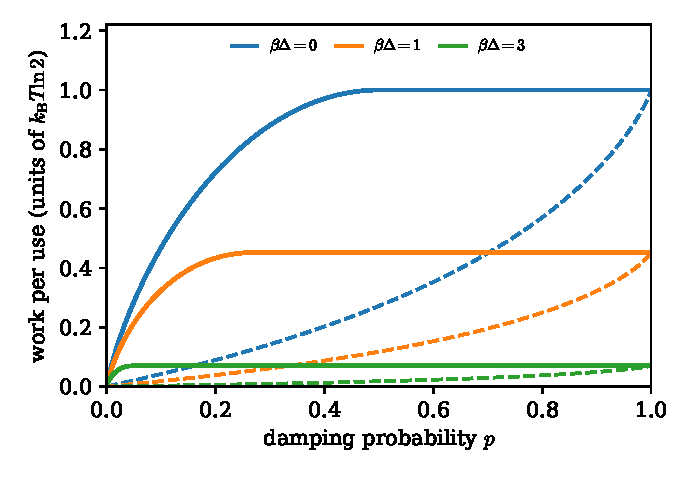
\includegraphics[width=0.62\linewidth]{fig-damping.pdf}
\caption{Work per use of amplitude damping with probability $p$, in real time (solid) and in batch (dashed), at three values of $\beta\Delta$. The curves meet only at $p=0$ and at full reset, $p=1$. Beyond $p=1/(1+e^{\beta\Delta})$ the real-time cost equals the cost of a full reset.}
\label{fig:damping}
\end{figure}

The real-time formula has a striking consequence. Maximizing $h(y)-\beta\Delta y/\ln 2$ over all $y$ gives $y=1/(1+e^{\beta\Delta})$ and the value $\log_2(1+e^{-\beta\Delta})$, which is the cost of a full reset. So once $p\ge1/(1+e^{\beta\Delta})$, a partial reset costs exactly as much as a full one in real time (Figure~\ref{fig:damping}). In batch, the cost of a partial reset rises smoothly to that value and reaches it only at $p=1$.

\paragraph{A finite example.} At one point the real-time cost can be met by a small explicit device. Take $p=1/2$ and $\beta\Delta=\ln2$. Since $p\ge1/(1+e^{\beta\Delta})$, the real-time cost is that of a full reset, $\log_2(3/2)$ bits or about $0.585\,\Delta$ per use, and the device never has to recover anything. Before the first input it prepares one ground-state qubit of gap $\Delta$ per use, and in round $t$ it applies the conserving rotation $|10\rangle\mapsto(|10\rangle+|01\rangle)/\sqrt2$ to the input and the $t$-th prepared qubit. The preparation uses only ordinary thermal qubits. Pool the $n$ memory qubits, initially thermal, with $R$ reservoir qubits of the same gap, and let a battery qubit of gap $w\Delta$ start excited. The $k$-excitation shell of the pool has dimension $\binom{R+n}{k}$. Whenever $\binom{R}{k+w}\ge\binom{R+n}{k}$, one energy-conserving permutation moves the whole shell onto states with every memory in its ground state, the reservoir in shell $k+w$ and the battery lowered; the other shells are left alone. The ratio $\binom{R}{k+w}/\binom{R+n}{k}$ decreases in $k$, so the preparation fails exactly on an upper tail of $\mathrm{Bin}(R+n,1/3)$. Because it happens before any input, its failure probability bounds the error against every adaptive observer once, not once per round. After the last output each memory is swapped with a fresh thermal qubit of the same gap, which returns the controller exactly on every branch. Table~\ref{tab:finite} gives exact values for $n=100$. With $R=n^2$ and $w=n\log_2(3/2)+O(\sqrt{\ln n})$ the error is at most $n^{-2}$ for $n\ge1000$, by Hoeffding's inequality. The preparation is one large nonlocal permutation, not an efficient circuit.

\begin{table}[t]
\centering
\begin{tabular}{rrrrr}
reservoir $R$ & qubits & work & per use & error at most\\\hline
2{,}000  & 2{,}208  & $118\Delta$ & $1.18\Delta$ & $0.00999$\\
10{,}000 & 10{,}208 & $70\Delta$  & $0.70\Delta$ & $0.00548$\\
50{,}000 & 50{,}208 & $63\Delta$  & $0.63\Delta$ & $0.00156$
\end{tabular}
\caption{Real-time amplitude damping with $p=1/2$ at $\beta\Delta=\ln2$, for $n=100$ uses; the asymptotic cost is $0.585\Delta$ per use. The qubit count includes the reservoir, 100 memories, 100 fresh thermal qubits for the final swaps, a 7-qubit round counter and the battery. The battery drops by the stated work with probability one minus the error and is otherwise untouched. Errors are exact binomial tails, rounded up.}
\label{tab:finite}
\end{table}

\paragraph{A finite saving.} The same example shows the batch saving at a finite size. At $p=1/2$ and $\beta\Delta=\ln2$ the batch capacity is about $0.154\,\Delta$ per use, against $0.585\,\Delta$ in real time, but batch constructions approach it only slowly. Fix the error at $10^{-8}$, and allow the controller to lose at most $10^{-5}\Delta$ of free energy, the battery to end with at most $10^{-5}$ bits of entropy, and its mean energy to differ from the nominal level by at most $10^{-5}\Delta$. Every real-time implementation of $234$ uses then has nominal work above $132.109\,\Delta$. This is~\eqref{eq:converse} with the estimate of Appendix~\ref{app:invertible} at the input with excited population $16/25$, where $\|(\Phi^c)^{-1}\|_\diamond=3$, less the three budgets. Only product inputs are used, so the bound also holds under the batch error criterion. A batch implementation does better. It prepares $234$ pure environment qubits for $137\Delta$ and runs the conserving partial swap of the real-time device. Before releasing the outputs it swaps the used environment into one of $32$ fresh thermal copies, chosen by a thermal five-qubit register, and then locates it again from the outputs, a position decoder as in~\cite[Sec.~7]{FBB21}. This purifies the register and returns $5\Delta$, so the nominal work is $137\Delta-5\Delta=132\Delta$, with error below $8.71\times10^{-9}$. At $256$ uses the same construction prepares the environments for $150\Delta$ and returns $11\Delta$ from $2^{11}$ positions: nominal work $139\Delta$ against a real-time bound of $144.53\Delta$, a saving above $5.5\Delta$. The saving needs the error: at zero error, the estimate of Appendix~\ref{app:invertible} applied to the whole block gives a batch device the same bound as real time, as in the exact row of Theorem~\ref{thm:werner}. The reservoirs that run the preparation and the refund are astronomically large, so this certifies that waiting saves work at a definite finite size, not that the saving is practical.

\section{The Werner--Holevo channel}\label{sec:werner}

The Werner--Holevo channel $W(\rho)=(\Tr(\rho)\,I-\rho^T)/2$ on a qutrit is the standard example of a unital channel that is not a mixture of unitaries~\cite{LandauStreater93}. It is not even factorizable~\cite[Ex.~3.1]{HaagerupMusat11}, so it is not a limit of noisy operations. Its Choi state is the normalized projector onto the antisymmetric subspace of two qutrits. The isometry
\[
V|i\rangle=\tfrac{1}{\sqrt2}\sum_{j,k}\epsilon_{ijk}\,|j\rangle|k\rangle
\]
is a Stinespring dilation in which output and environment play symmetric roles, so $W$ is its own complementary channel. And $W$ is invertible, with $W^{-1}(Y)=\Tr(Y)\,I-2Y^T$.

\begin{proof}[Proof of Theorem~\ref{thm:werner}]
\emph{Real time.} By Lemma~\ref{lem:invertible}, $s_\rho(W)=S(W(\rho))$, which is at most $\log_2 3$ and equals it at $\rho=I/3$; so $\Trt(W)=\log_23$. Every exact real-time round on half of a maximally entangled pair adds exactly $\log_2 3$ bits of entropy to the device, whatever the device did before, and Lemma~\ref{lem:accounting} gives $w\ge n\log_23$. With an information battery, a device that applies $V$ with one pure qutrit of the battery per round, and swaps the used qutrit into a thermal cell, attains this. At error $\varepsilon$ the same argument, run through the bounded inverse and continuity of conditional entropy on the nine-dimensional system $QO$, gives
\[
w\ \ge\ \sum_{t=1}^n\bigl[\log_2 3-g_9\bigl(\min\{1,10\sqrt{\varepsilon}\}\bigr)\bigr]_+,\qquad g_D(t)=2t\log_2 D+(1+t)\,h\bigl(t/(1+t)\bigr),
\]
which is $n\log_2 3-O(\log n)$ at $\varepsilon=n^{-2}$.

\emph{Batch.} The batch rate is zero by the theorem of Faist, Berta and Brand\~ao, since $\Tcap(W)=0$ for a unital channel at zero Hamiltonian~\cite{FBB21}. Our earlier construction sharpens this~\cite{ImmediateDelivery}: a batch implementation at error $\varepsilon$ whose initial state is flat on $k$ levels of an $m$-level bath with $\log_2(m/k)\le2\log_2(1/\varepsilon)+2\log_2(n+1)+O(1)$. With the accounting of Section~\ref{sec:law} its free energy is at most $6\log_2 n+O(1)$ at $\varepsilon=n^{-2}$. For exact batch implementation, the joint output-reference state must lie in the support of the $n$-fold antisymmetric projector, on which the partial trace acts as the invertible map $W^{\otimes n}$. The argument of Lemma~\ref{lem:invertible} then forces $w\ge n\log_23$, attained by the same pure qutrits.
\end{proof}

No exact implementation can end with a sharp mechanical battery: each exact round triples the rank of the device, so if the controller returns, a battery that starts pure must end with rank at least $3^n$. This is why the exact entries of Theorem~\ref{thm:werner} are stated for free energy.

The bound in the real-time part is measurable. Let $\delta$ be the average probability that the output and the reference of a round fail a two-outcome test for the antisymmetric subspace. Any real-time implementation, of any size and with any memory, then draws at least $n[\log_2 3-g_9(\min\{1,10\sqrt{\delta}\})]_+$ bits of free energy (Appendix~\ref{app:werner}). We return to this in Section~\ref{sec:discussion}.

The zero-error obstruction of Theorem~\ref{thm:werner} holds for every extreme channel. A channel is extreme in the convex set of channels when the products $A_i^*A_j$ of its minimal Kraus operators are linearly independent~\cite{Choi75}; Werner--Holevo and amplitude damping with $0<p<1$ are examples.

\begin{proposition}[At zero error, waiting saves nothing for extreme channels]\label{prop:extreme}
Let $\Phi$ be extreme with complementary channel $\Phi^c$, and let
\[
a_\beta(\Phi)=\max_\rho\Bigl[S(\Phi^c(\rho))+\tfrac{\beta}{\ln2}\Tr H\bigl(\Phi(\rho)-\rho\bigr)\Bigr].
\]
Every implementation of $n$ uses with zero error, in batch or in real time, draws at least $n\,a_\beta(\Phi)-o(n)$ bits of free energy from its battery and controller. For extreme channels $a_\beta(\Phi)=\Trt(\Phi)$, so at zero error a batch device pays the full real-time rate.
\end{proposition}

The proof is in Appendix~\ref{app:extreme}: extremality makes the branches of any exact implementation orthogonal, so the device's entropy rises by exactly the entropy of the complementary output, whatever its initial state.

For amplitude damping at $p=1/2$ and $\beta\Delta=\ln2$, the asymptotic separation between $0.585\,\Delta$ per use in real time and the batch capacity $0.154\,\Delta$ therefore exists only because some error is tolerated. The finite constructions of Section~\ref{sec:classical} certify smaller savings, at their stated block sizes and error budgets.

\section{What is free}\label{sec:free}

A \emph{thermal operation} at $(H,\beta)$ is a channel $\rho\mapsto\Tr_BU(\rho\otimes\gamma_B)U^*$, where the bath $B$ (not the battery of Section~\ref{sec:setting}) is finite-dimensional with an arbitrary Hamiltonian $H_B$, $\gamma_B$ is its Gibbs state at the same $\beta$, and $U$ commutes exactly with $H\otimes I+I\otimes H_B$~\cite{Janzing00,HorodeckiOppenheim13,Brandao13,vomEnde22,LieEtAl26}. We impose no large-bath conditions. The set is not closed~\cite{vomEnde22}, and by a limit of thermal operations we mean a point of its closure. \emph{Enhanced thermal operations} are the time-covariant channels that preserve $\gamma$~\cite{Cwiklinski15}.

Which processes are free? We call a process \emph{free in batch} (\emph{in real time}) if its optimal batch (real-time) work rate is zero, at vanishing error. Thermal operations, energy-conserving unitaries with a Gibbs bath, are the standard model of free dynamics~\cite{Janzing00,HorodeckiOppenheim13,Brandao13}. They preserve the Gibbs state and commute with time evolution~\cite{Lostaglio15}. Gibbs-preserving maps~\cite{Janzing00,FDOR15,FR18} are strictly more powerful: they can even create coherence between energy levels~\cite{FOR15}. The time-covariant ones, called enhanced thermal operations~\cite{Cwiklinski15}, coincide with the closure of the thermal operations for a qubit~\cite{Cwiklinski15,vomEnde22}, but not for a qutrit~\cite{Cwiklinski15,DingFengHu21}. By the theorem of Faist, Berta and Brand\~ao, a time-covariant process is free in batch exactly when it is an enhanced thermal operation (see below). In real time the answer is the thermal operations.

\begin{theorem}[What is free in real time]\label{thm:free}
Let $\Phi$ be any channel on a system with Hamiltonian $H$, at any temperature. Then $\Trt(\Phi)=0$ if and only if $\Phi$ lies in the closure of the thermal operations.
\end{theorem}

Lie, Son, Boes, Ng and Wilming showed that a channel that fixes the Gibbs state is a thermal operation exactly when some dilation, with no energy conservation or thermal bath assumed, also leaves its environment unchanged when the input is the Gibbs state; energy conservation, a thermal bath and time covariance then follow~\cite[Prop.~4]{LieEtAl26}. Theorem~\ref{thm:free} is a robust, work-cost form of their criterion. As in their exact case, zero cost forces time covariance and only the Gibbs input matters; here the bounds do not depend on the size of the bath, and this is what characterizes the closure.

So the enhanced thermal operations that are not limits of thermal operations are exactly the time-covariant processes that are free in batch but cost work in real time. This set is known to be nonempty. At zero Hamiltonian it contains the Werner--Holevo channel, which is not factorizable~\cite[Ex.~3.1]{HaagerupMusat11} and which Faist, Oppenheim and Renner cite as a unital map that is not a thermal operation~\cite{FOR15}, and for an equally spaced qutrit a channel of Ding, Ding and Hu~\cite{DingFengHu21}. We price both: $\log_23$ bits per use for the first (Theorem~\ref{thm:werner}), and an explicit positive cost, at every gap ratio and temperature, for a family that contains the second (Proposition~\ref{prop:qutrit}). For that family a single input state already separates the channel from every limit of thermal operations, with no assumption on the bath; Ding, Ding and Hu proved this for equally spaced levels, under assumptions on the bath and the temperature.

\paragraph{Batch.} For time-covariant $\Phi$ the batch cost is $\Tcap(\Phi)=\max_\rho[D(\Phi(\rho)\|\gamma)-D(\rho\|\gamma)]$, in relative-entropy form. The value at $\rho=\gamma$ is $D(\Phi(\gamma)\|\gamma)\ge0$, and by monotonicity of relative entropy every value is at most zero when $\Phi(\gamma)=\gamma$. So $\Tcap(\Phi)=0$ exactly when $\Phi$ is an enhanced thermal operation, and by the theorem of Faist, Berta and Brand\~ao such a process can be run in batch at vanishing work per use~\cite{FBB21}. This is a direct consequence of their work; we record it only for contrast. Faist, Oppenheim and Renner ask whether thermal operations aided by a time reference can do everything Gibbs-preserving maps can~\cite{FOR15}, and Tajima and Takagi showed that for some Gibbs-preserving maps no finite amount of coherence suffices~\cite{TajimaTakagi25}. For a device that carries its own phase reference and must return it, a Gibbs-preserving channel is free in batch exactly when its energy change lies in the span of the products of its Kraus operators; some non-covariant Gibbs-preserving channels are free and others cost work~\cite{KeepingTime}.

\paragraph{Real time: thermal operations are free.} Let $\Phi$ be a thermal operation with bath $(H_B,\gamma_B)$. Its dilation is an exact extension in Definition~\ref{def:rtcost}, with the bath purifier as $F$. Energy conservation and the Gibbs identity give, for every input,
\[
s_\rho(\Phi)+\tfrac{\beta}{\ln2}\Tr H\bigl(\Phi(\rho)-\rho\bigr)\ \le\ -D\bigl(\Gamma(\rho)\,\big\|\,\gamma_B\bigr)\ \le\ 0,
\]
where $\Gamma(\rho)$ is the bath output. So $\Trt(\Phi)=0$. If $\Phi$ is only a limit of thermal operations $\Phi_k$, the dilation of $\Phi_k$ is a feasible extension for $\Phi$ at error $\varepsilon$ once $\Phi_k$ is $\varepsilon$-close to $\Phi$, so the same bound holds for $s_{\rho,\varepsilon}(\Phi)$ up to an energy correction of order $\beta\varepsilon\,\mathrm{span}(H)$. Letting $\varepsilon\to0$, every limit of thermal operations has zero real-time cost as well. Operationally this is the obvious statement that a device using one fresh thermal bath per round runs a thermal operation in real time at no cost.

\paragraph{Real time: only thermal operations are free.} The converse is the substance of Theorem~\ref{thm:free}. For baths of bounded size it follows from compactness and the exact characterization of Lie et al.~\cite{LieEtAl26}, but a small real-time cost may be achieved only with baths of unbounded size and arbitrarily small eigenvalues. We prove it in four steps (Appendix~\ref{app:zero-set}).
\begin{enumerate}[label=(\roman*)]
\item Since $\Trt(\Phi)\ge D(\Phi(\gamma)\|\gamma)$, zero cost forces $\Phi(\gamma)=\gamma$. It also supplies dilations whose \emph{Gibbs defect} $G=D\bigl(U(\gamma\otimes\tau)U^*\,\big\|\,\gamma\otimes\omega\bigr)$ tends to zero, where $\omega$ is the bath output on input $\gamma$. The defect is the relative entropy between the joint output and the product of the Gibbs state with the bath output; it vanishes exactly for the equilibrating dilations of Lie et al., up to a unitary on the bath.
\item A small Gibbs defect forces time covariance. This is a robust form of Proposition~4 of~\cite{LieEtAl26}: the dilation nearly commutes with $(\gamma\otimes\tau)^{iz}$, the time evolution of $H+H_B$ with $H_B=-\beta^{-1}\ln\tau$, with a bound that involves neither the bath dimension nor its smallest eigenvalue.
\item A replacement theorem turns any dilation of a time-covariant channel with small defect $G$ into a finite thermal operation within $c_{H,\beta}\,G^{1/(6\max\{1,r\})}$ in diamond norm, where $r$ is the number of rationally independent energy gaps of $H$. The new thermal operation generally has a different bath.
\item Irrational energy gaps are approximated by commensurate ones with the same integer labels, and a finite thermal lattice absorbs the difference so that the original Hamiltonian is conserved exactly. This handles the accidental gap coincidences at which thermal operations depend discontinuously on $H$~\cite[Sec.~III]{vomEnde22}. No external phase reference is used.
\end{enumerate}
As in the exact criterion of Lie et al., only the Gibbs input matters: $\Phi$ is a limit of thermal operations exactly when $\Phi(\gamma)=\gamma$ and the real-time entropy cost at the Gibbs input vanishes. Lie et al.\ also observe that an enhanced thermal operation outside the thermal operations must change its environment even at the Gibbs input, so its environment must hold non-equilibrium free energy, which may be depleted~\cite{LieEtAl26}. The real-time entropy cost $s_\gamma(\Phi)$ is the least such change, and in real time it is paid in work.

Two remarks on the controller. The controller acts as a catalyst that is returned only at the end and may be correlated with past outputs; it does not enlarge the free set, because those correlations only add to the cost in Lemma~\ref{lem:accounting} and its free energy must return up to $o(n)$, which also excludes the embezzlement that a catalyst returned only approximately would otherwise allow~\cite{FOR15}. And since the lower bound of Section~\ref{sec:law} holds for any controller, Theorem~\ref{thm:free} bears on the time-reference question of Faist, Oppenheim and Renner~\cite{FOR15}: a phase reference that the device must return, up to $o(n)$ free energy, cannot make a non-covariant Gibbs-preserving map free in real time. A reference that is used up and paid for is not covered.

\paragraph{A clock that returns cannot help.} If the controller returns exactly, as in our constructions of time-covariant channels, and the battery is stationary, a non-covariant channel cannot be run at vanishing error, whatever work is spent~\cite{MarvianSpekkens19,LostaglioMuller19}. The following proposition makes this quantitative.

\begin{proposition}[A returning clock]\label{prop:clock}
Suppose the controller returns exactly to $\alpha_C$, independent of all other systems, and the battery is stationary. Let $J_\Phi$ be the normalized Choi state of $\Phi$ and $G=H_O-H_I^T$, where $H_I=H_O=H$ act on the input and output. Then, in real time or in batch and whatever work is drawn, every implementation of $n$ uses of $\Phi$ has error at least
\[
\tfrac14\sup_t\bigl\|J_\Phi-e^{-\mathrm itG}J_\Phi e^{\mathrm itG}\bigr\|_1,
\]
which is positive exactly when $\Phi$ is not time-covariant. For the Hadamard gate on a qubit with $H=E|1\rangle\langle1|$ the error is at least $1-2^{-n}\binom{n}{\lfloor n/2\rfloor}$, which tends to one.
\end{proposition}

\begin{proof}
Fix an observer whose inputs, together with the systems it keeps, are invariant under time evolution; the initial reservoir states are invariant too, and so is the battery's, because it is stationary. Composing every operation of the device, including its final clean-up, and tracing out everything except the controller and a set $Y$ of systems we keep, gives a channel $\Lambda$ from $C$ to $CY$ that commutes with time evolution. Exact return means $\Lambda(\alpha)=\alpha\otimes\rho$. Write $x_t$ for a state evolved for time $t$. Covariance gives $\Lambda(\alpha_t)=\alpha_t\otimes\rho_t$, and since fidelity does not decrease under $\Lambda$ and is multiplicative on products, $f(\alpha,\alpha_t)\le f(\alpha,\alpha_t)f(\rho,\rho_t)$. For small $t$ the fidelity $f(\alpha,\alpha_t)$ is positive, so $\rho_t=\rho$, and by the group law this holds for every $t$. So the final state of everything we keep is invariant in time: a controller cannot pass on asymmetry and keep it, which is the no-broadcasting theorem for asymmetry~\cite{MarvianSpekkens19,LostaglioMuller19}.

For the first bound, let the observer send half of a maximally entangled state in the first round, and $|0\rangle$ in every later round, and keep the other half as a reference with Hamiltonian $-H^T$, so that the pair is invariant. The first output and the reference end in a state $J'$ that commutes with $G$, so $\|J_\Phi-e^{-\mathrm itG}J_\Phi e^{\mathrm itG}\|_1\le2\|J_\Phi-J'\|_1$ for every $t$, and the observer distinguishes $J'$ from $J_\Phi$ with advantage $\tfrac12\|J_\Phi-J'\|_1$. For the Hadamard gate, send $|0\rangle$ in every round. The outputs end in a state that commutes with the total energy, while the ideal output $|+\rangle^{\otimes n}$ has weight $2^{-n}\binom nk$ in the sector with $k$ excitations. So the real output passes the test for $|+\rangle^{\otimes n}$ with probability at most $\max_k2^{-n}\binom nk$, and the ideal one with probability one.
\end{proof}

The battery must be stationary. A battery in a broad superposition of energy levels is a phase reference of its own, and the device may spend it while the controller returns exactly. Let the battery be a ladder with spacing $E$, prepared in a sine-shaped wave packet on $L$ consecutive levels with $n+1$ empty levels on each side, and let each use apply the Hadamard gate to every pair $\{|0\rangle|q\rangle,|1\rangle|q-1\rangle\}$ of equal total energy, and the identity on the two unpaired states at the edges. This unitary conserves energy. Because the packet barely changes when it is shifted by one level, each use acts as the Hadamard gate up to $\pi/(\sqrt2(L+1))$ in strategy distance, whatever the observer does. With $L=n^3$ and a trivial controller, $n$ uses have error $O(n^{-2})$, while the battery's entropy changes by at most $\log_2(L+2n+2)=o(n)$. The battery's coherence is spent, not broadcast, so this is consistent with the no-broadcasting theorem; it shows that every initial store of asymmetry, a coherent work store included, must be counted as part of the controller.

\paragraph{A clock that returns approximately.} Theorem~\ref{thm:clock} relaxes the return condition. A controller \emph{returns approximately} if, uniformly over observers, its final joint state with all other systems is within $\eta_n\to0$ in trace distance of $\alpha_C$ tensored with their final state, and its mean energy and its entropy change by $o(n)$. This is the return condition of our lower bounds, with closeness of the joint state added. Trace-distance closeness alone would not suffice: a broad reference can hand over energy of order $n$ while staying close to its initial state, and would then act as a second battery. The controller may start with any declared amount of phase reference.

\begin{theorem}[A clock that returns approximately]\label{thm:clock}
Let $\Phi$ be any channel. Suppose the controller need only return approximately: its final joint state with everything else is close to its initial state tensored with the rest, and its mean energy and its entropy change by $o(n)$. Then the optimal real-time work per use at vanishing error is $\kB T\ln2\,\Trt(\Phi)$, with deterministic work. For a unitary $U$ it is exactly the largest eigenvalue of $U^*HU-H$, and the battery reaches its target on every branch. If $U$ is not time-covariant, the heat baths of any such implementation with deterministic work must have a total energy range that grows faster than $n$.
\end{theorem}

Faist, Berta and Brand\~ao leave open whether thermal operations can implement every i.i.d.\ channel that is not time-covariant at its thermodynamic capacity, and expect this to need a very large amount of coherence, as the reverse Shannon theorem needs embezzling states~\cite{FBB19},~\cite[Sec.~9]{FBB21}. Theorem~\ref{thm:clock} settles the real-time form of this question: a clock that returns approximately runs every channel at the optimal real-time rate, and the coherence it needs is indeed large. In batch, a clock that must return in the same sense, which rules out embezzlement, cannot always reach the capacity: for qubit dephasing in the $X$ basis, batch costs as much as real time, more than the capacity, and the batch cost of every channel with a returned clock is given in~\cite{KeepingTime}. The coherence is invested, not consumed. The operating work is the same formula, while for a gate the clock pays in capital~\cite{ChiribellaYangRenner21,TSS20} and the baths in energy range, and the controller's energy comes back only on average, not branch by branch~\cite{KeepingTime}. Channels that are not gates can need far less: a Gibbs-preserving qubit channel that only creates coherence runs in batch at its capacity, zero, with a clock whose energy spreads like $\sqrt n$~\cite{KeepingTime}.

The lower half of Theorem~\ref{thm:clock} is the bound of Section~\ref{sec:law}, which uses neither time covariance nor exact return. The construction (Appendix~\ref{app:clock}) rests on one primitive. Let $D=U^*HU-H$, $w$ its largest eigenvalue and $B=wI-D\ge0$. A thermal qubit with a large gap $M$ can absorb the energy $B$ by a rare excitation: a rotation between the payload and this qubit, by the angle whose sine is $\sqrt{B/M}$, changes the payload channel by only $O(\|B\|/M)$, yet the qubit takes up exactly the input-dependent part of the energy change, on average. What remains is the constant $w$, which a sharp battery supplies. Lifting the whole contact with a phase reference makes it conserve energy exactly, and the reference's energy then drifts by $O(1/M)$ as an operator, whatever the input. For the Hadamard gate on a qubit with $H=E|1\rangle\langle1|$, this gives work exactly $nE/\sqrt2$, with error and return error $O(n^{-3})$. For a general channel the same primitive is applied to a dilation whose bath carries the Hamiltonian $-\beta^{-1}\ln\zeta$, with $\zeta$ the bath state at the worst input. This turns the bath's entropy into energy, so one operator inequality handles the entropy and energy terms together. The bath copies are prepared in their source state, and everything used to prepare them is returned, by the finite-source module of the companion paper on processes~\cite[Lemma~12]{Answering}, applied with one slot.

The energy-conserving lift and the reusable reference go back to {\AA}berg~\cite{Aberg14}. Repaying a reference's drift with work is due to Korzekwa, Lostaglio, Oppenheim and Jennings~\cite{KLOJ16}, and forming coherent sources at their free-energy cost to~\cite{Brandao13,KLOJ16}. The rare-excitation primitive and the work rate for every channel appear to be new. The bound on the baths' range is an argument of Wigner--Araki--Yanase type, of the kind that bounds the energy and coherence a reference needs to implement a gate~\cite{ChiribellaYangRenner21,TSS20}; what is new is that, with deterministic work and a controller that returns, it falls on the heat baths. Faist, Berta and Brand\~ao already observed that for such channels the environment must coherently compensate the energy differences between inputs~\cite{FBB19}; the bound makes this quantitative.

\paragraph{The clock is expensive.} Theorem~\ref{thm:clock} makes the operating work the formula, but the clock is not cheap. Unlike a circuit acting on one register, whose energy requirement need not grow with its depth~\cite{ChiribellaYangRenner21}, $n$ uses on fresh systems call for $n$ times the asymmetry. In a companion paper we show that, for a gate, its initial free energy must grow at least like $n/(\varepsilon+\eta)$, where $\eta$ is the return error, a quantitative form of the trade-off between disturbing a reference and the asymmetry it can impart~\cite{MarvianSpekkens19}, that the range of its baths and the strength of their interactions must grow at least like $n/\sqrt\varepsilon$, and that its energy comes back only on average, through a lottery of rare large transfers~\cite{KeepingTime}.

At zero Hamiltonian a thermal operation is a mixture of noisy operations, unitaries acting with a maximally mixed bath~\cite{HHO03}. Lie et al.\ note that these mixtures are the strongly factorizable channels, and show that these are exactly the unital channels with an equilibrating dilation~\cite[Eq.~(14)]{LieEtAl26}, and their closure is the closure of the channels that factor through a finite-dimensional algebra with a faithful trace~\cite{MullerHermesPerry,ClosedMemory}. So at zero Hamiltonian Theorem~\ref{thm:free} says that real-time freeness is finite factorizability, as in our earlier work~\cite{Memory}.

\paragraph{The gap.} For a qubit, enhanced thermal operations coincide with the closure of the thermal operations~\cite{Cwiklinski15},~\cite[Thm.~10]{vomEnde22}. For a qutrit they do not, already for state transitions: exactly~\cite{Cwiklinski15} and approximately~\cite{DingFengHu21}. By Theorem~\ref{thm:free}, the difference is exactly the set of time-covariant processes that are free in batch but cost work in real time. At zero Hamiltonian it contains the Werner--Holevo channel, at a cost of $\log_2 3$ bits per use. At nonzero Hamiltonian it contains the following qutrit channels.

\begin{proposition}[A Gibbs-preserving process that is not free in real time]\label{prop:qutrit}
Let $H=\mathrm{diag}(0,E_1,E_2)$ with $0<E_1<E_2$, let $\lambda=e^{-\beta E_2}$, and let $\Phi$ have Kraus operators $\mathrm{diag}(\sqrt{1-\lambda},1,0)$, $\sqrt\lambda\,|2\rangle\langle0|$ and $|0\rangle\langle2|$. Then $\Phi$ is an enhanced thermal operation, so $\Tcap(\Phi)=0$, but
\[
\Trt(\Phi)\ \ge\ g_1\log_2\frac{1}{1-g_2}\ >\ 0,
\]
where $(g_0,g_1,g_2)$ are the Gibbs populations. Moreover, for the input $\psi_0=(|0\rangle+|1\rangle)/\sqrt2$ and every limit of thermal operations $\Theta$,
\[
\tfrac12\bigl\|\Theta(\psi_0)-\Phi(\psi_0)\bigr\|_1\ \ge\ \delta(\lambda)=\frac{(1-\lambda)\Delta_\lambda^2}{4(1-\lambda)\Delta_\lambda+2\lambda\bigl(1+2\sqrt{1-\lambda}\bigr)},\qquad\Delta_\lambda=\sqrt{1-\lambda}-(1-\lambda)>0.
\]
In particular $\Phi$ is at half diamond distance at least $\max\{\delta(\lambda),u^2/(2c^2)\}$ from the closure of the thermal operations, where $u=g_1g_2$ and $c=2+6u/\sqrt{1-\lambda}$.
\end{proposition}

The channel leaves level $1$ untouched, resets level $2$ to the ground state, and excites the ground state with probability $\lambda$, while keeping the coherence between levels $0$ and $1$ as large as positivity allows. The proof shows that the bath must end in orthogonal states after leaving level $1$ alone and after resetting level $2$. At the Gibbs input this forces correlations between bath and output worth at least $g_1\log_2\frac1{1-g_2}$ bits.

For equally spaced levels this is the enhanced thermal operation that Ding, Ding and Hu use (their Eq.~(11) with the transition matrix of their Eq.~(17)). It saturates the coherence bounds of~\cite{Cwiklinski15,Lostaglio15}. They proved that its output on $\psi_0$ cannot be approximated by any thermal operation acting on that input~\cite{DingFengHu21}, for equally spaced levels, bath degeneracies that grow with energy as in~\cite{HorodeckiOppenheim13}, and a range of temperatures. Proposition~\ref{prop:qutrit} removes all three assumptions and bounds the trace distance explicitly. Their bound is stated for perturbations of transition probabilities, so the two constants are not directly comparable.

The single-input bound rests on a law for thermal operations that may be of independent interest (Lemma~\ref{lem:coherence}). If a thermal operation moves the ground state to level $2$ with probability $T_{20}$, then $T_{20}\le\lambda$, and the coherence it keeps between levels $0$ and $1$ is at most $\frac12\bigl[1-\lambda+\sqrt{\lambda(\lambda-T_{20})}\bigr]$. The reason is that the bath can give up the energy $E_2$ only from states of total Gibbs weight at most $\lambda$. Moving the full probability $\lambda$ to level $2$ therefore forces an all-or-nothing transfer on those states, while $\Phi$ acts as if every state of the bath contributed the same partial amplitude $\sqrt\lambda$. With $T_{20}=\lambda$, $\Phi$ keeps the coherence $\sqrt{1-\lambda}/2$, above the bound by $\Delta_\lambda/2$.

\section{Undecidability}\label{sec:undecidable}

Our last result concerns generalized dephasing channels, also called Schur multiplier channels: $\Phi(\rho)=M\circ\rho$, the entrywise product with a positive semidefinite matrix $M$ that has unit diagonal.

\begin{theorem}[Undecidability]\label{thm:undecidable}
There is a dimension $d_0$ with the following property. For every $d\ge d_0$, every Hamiltonian on $\mathbb C^d$ that is diagonal in the dephasing basis and every temperature, no algorithm decides whether a generalized dephasing channel on $\mathbb C^d$ with cyclotomic entries is free in real time. The set of such channels that are free is not recursively enumerable.
\end{theorem}

By Theorem~\ref{thm:free}, free in real time means a limit of thermal operations; on these channels the easy direction of Theorem~\ref{thm:free} is enough (Section~\ref{sec:undecidable}). In batch the same question is trivial: a generalized dephasing channel preserves every energy population, hence the Gibbs state, so it is always free in batch. Our earlier work showed that the zero-Hamiltonian question is undecidable when the dimension may grow~\cite{Flagship}; Theorem~\ref{thm:undecidable} settles the fixed-dimension question left open there.

On dephasing channels the Hamiltonian and the temperature drop out. Being free in real time becomes a question about which Gram matrices of unitaries finite-dimensional algebras can approximate, and that question is undecidable at a fixed size by the work of Fu, Miller and Slofstra.

\begin{proof}[Proof of Theorem~\ref{thm:undecidable}]
\emph{Step 1: on dephasing channels, free means finitely factorizable.} Let $\Phi(\rho)=M\circ\rho$ be a generalized dephasing channel, and let the Hamiltonian be diagonal in the same basis. Then $\Phi$ preserves every energy population, so the energy term vanishes and $\Trt(\Phi)=\sup_\rho s_\rho(\Phi)$, the zero-Hamiltonian purity cost of our earlier work. That cost vanishes exactly when $\Phi$ is a limit of channels that factor through finite-dimensional algebras with a faithful trace~\cite{Memory,ClosedMemory}. For dephasing channels these are the limits of channels with $M_{ij}=\tau(u_j^*u_i)$ for unitaries $u_i$ in a finite-dimensional algebra $\mathcal N$ with faithful trace $\tau$~\cite{HaagerupMusat11,Musat25}. Each such channel is a thermal operation. Write $\mathcal N=\bigoplus_k M_{n_k}$ with $\tau=\sum_kw_k\tr_{n_k}$ (normalized traces), give the bath the Hamiltonian $H_B=\bigoplus_kE_kI_{n_k}$ with $e^{-\beta E_k}=w_k/n_k$, so that its Gibbs state is the density of $\tau$, and use $U=\sum_i|i\rangle\langle i|\otimes u_i$. This $U$ commutes with $H\otimes I+I\otimes H_B$, its bath starts in the Gibbs state, and it implements $\Phi$. (This is the dilation used for Schur multipliers in~\cite{HaagerupMusat11,LieEtAl26}, with the bath Hamiltonian read off from the trace as in~\cite{LieEtAl26}.) Conversely, every limit of thermal operations has zero real-time cost (Section~\ref{sec:free}). So a dephasing channel is a limit of thermal operations exactly when it is a limit of finitely factorizable channels, at every temperature and for every Hamiltonian diagonal in its basis. This step does not use the hard direction of Theorem~\ref{thm:free}.

\emph{Step 2: the reduction.}
\begin{enumerate}[label=(\alph*), leftmargin=*]
\item For a recursively enumerable but not recursive set $X$, Fu, Miller and Slofstra give a number $N$ of questions, eight answers, and a computable map from $n$ to finite lists of real tables with cyclotomic entries: if $n\in X$ none of them is a commuting-operator correlation, and if $n\notin X$ one of them is an approximately quantum synchronous correlation~\cite[Thm.~7.2]{FMS}. Exact tests discard every table that is not a synchronous correlation (Appendix~\ref{app:fixeddim}).
\item Approximately quantum synchronous correlations are exactly those realized by projections in an ultrapower of the hyperfinite factor~\cite{KPS18}.
\item The construction of Musat and R{\o}rdam turns such projections into unitaries in the same algebra with a prescribed Gram matrix~\cite{MusatRordam}.
\item The corresponding dephasing channel on $\mathbb C^{d_0}$, $d_0=16N+1$ (the identity, the $8N$ symmetries $2p_j-1$ and the $8N$ unitaries $(2p_j-1+i)/\sqrt2$), is a limit of finitely factorizable channels exactly when its Gram matrix is a limit of finite-dimensional ones~\cite{Musat25}. Repeating indices embeds it in every dimension $d\ge d_0$.
\end{enumerate}
The entries lie in cyclotomic fields: the construction of Fu, Miller and Slofstra uses sines and cosines of rational multiples of $\pi$ and finite group-algebra coefficients~\cite[Sec.~7, Thm.~7.2]{FMS}, and the transfer to unitaries adds only $i$ and $\sqrt2$. The field grows with $n$; no fixed number field is claimed. So each channel is a finite, exact input. Appendix~\ref{app:fixeddim} gives the reduction in full: the faithful Gram transfer, the exact filters on the tables, and the padding to larger dimensions. Program $n$ never halts exactly when some channel in its list is free; when it halts, no channel in the list is even factorizable. If the free channels were recursively enumerable, the non-halting programs would be too, which is impossible.\footnote{The reduction asks whether at least one channel in a finite list is free, so it is a disjunctive truth-table reduction from the complement of the halting problem rather than a many-one reduction. The dimension $d_0=16N+1$ is not explicit, because Fu, Miller and Slofstra do not give $N$ explicitly.}
\end{proof}

\section{Discussion}\label{sec:discussion}

\paragraph{Order, not speed.} The excess work of finite-time thermodynamics disappears when a process runs slowly enough. The surcharge here does not. Our rates allow devices of any size and any running time, so the gap between $\Trt$ and $\Tcap$ survives arbitrarily slow operation. It is a cost of order: an operation becomes more expensive, without being performed faster, because some of its outputs must become unavailable sooner.

\paragraph{A laboratory test.} The Werner--Holevo bound needs no knowledge of the device beyond our accounting: declared reservoirs, a mechanical battery and a controller that returns. Feed each round one half of a maximally entangled pair of qutrits, test the output and the kept half for the antisymmetric subspace, and record the average failure probability $\delta$. Every real-time implementation, of any size and with any memory, then draws at least $n[\log_2 3-g_9(\min\{1,10\sqrt\delta\})]_+$ bits of free energy from its battery and controller. With a mechanical battery whose entropy does not change and a returning controller, this free energy leaves as heat into the reservoirs (Lemma~\ref{lem:accounting}). A qutrit platform that implements the channel round by round must therefore warm its environment by nearly $\kB T\ln 3$ per use, whereas a batch implementation need not, in principle. The correction term is weak: the bound is informative only for $\delta$ below about $2\times10^{-4}$, and within ten percent of $\log_2 3$ only near $\delta=10^{-6}$. Sharpening it, and turning it into a protocol with confidence intervals, is a separate task.

\paragraph{Processes with memory.} Our results concern repeated uses of one channel. A process whose later steps depend on earlier inputs is different: if an earlier output must leave before a later input arrives, the device has to keep a record correlated with an output it has already released, and erasing that record afterwards costs work even when everything is classical. This is the online cost of classical agents~\cite{Thompson25}, and the modularity dissipation of classical computation, the loss of correlations with degrees of freedom that a local operation cannot act on, has the same form~\cite{BMC18}; agents that extract work efficiently must balance prediction against forgetting~\cite{Fiderer26}. Processes with several time steps that preserve thermal equilibrium have been characterized as the causally ordered thermal ones~\cite{Milz26}. The common principle is that the price of real time is the correlation a device must keep with outputs it has already released. For a repeated classical channel no such correlation is needed (Theorem~\ref{thm:classical}); for a quantum channel it can be forced (the term $m_\rho$); for a process with memory the task itself forces it.

\paragraph{Waiting a little.} For time-covariant channels, a device that may hold some outputs before releasing them sits between the two regimes. Running blocks of length of order $\log(n/\varepsilon)$ in batch, a delay that grows with the number of uses, already reaches the batch rate~\cite{TimeOrder}; the cost at a fixed latency is open. For other channels with a returned clock, the batch endpoint is the single-letter cost of~\cite{KeepingTime}, which can exceed $\Tcap$.

\paragraph{Open problems.} Our constructions use reservoirs of astronomical size; efficient reservoirs, and an autonomous engine with a time-independent Hamiltonian, are open. For channels that are not time-covariant, the batch cost with a returned clock is a single-letter quantity~\cite{KeepingTime}; whether it can be reached with modest reference capital is open. The constant $\delta(\lambda)$ in Proposition~\ref{prop:qutrit} is not optimal. Thermal operations built from partial swaps come within about $0.10\lambda$ of $\Phi(\psi_0)$ at low temperature and $(1-\lambda)/2$ at high temperature, and numerical searches find nothing closer; the exact distance is open. Finally, $\Trt$ is defined by an optimization whose zero set is undecidable; computable bounds for typical channels would make the law practical.

\section*{How this work was done}\addcontentsline{toc}{section}{How this work was done}
This paper is the work of its two authors together with AI models from more than one developer. The authors set the direction of the research throughout: they chose the questions, decided which lines to pursue and which to drop, judged and selected the results, and take full responsibility for every claim. The models did most of the exploration, derivation, computation and drafting.

Much of the exploration took place in long working sessions, in which many model instances worked on a problem in parallel, communicated with one another, and built on and challenged each other's results. We also set the models against one another. Before a result was kept, an instance that had not seen its proof, usually from a different developer, first tried to refute the statement and then audited the proof line by line, with exact computation wherever possible. Each paper then went through several rounds of adversarial review, on its own and together with its companion papers, and AI-assisted literature searches were used to check priority and how we report the work of others. Errors found at any of these stages are corrected in the text. The proofs are given in full: the checks support them but do not replace them.

Machine checks accompany the paper. Programs in its repository, \url{https://github.com/Apsiape/save-work-by-waiting}, check the numbers, worked examples and finite constructions listed in its verification notes, with exact arithmetic where possible, and test the stated inequalities on many random and near-extremal instances. The general theorems, and the construction and continuity arguments the notes do not list, are proved in the text; results quoted from the companion papers are checked in their own repositories. The finite and algebraic cores of the arguments are proved in Lean with Mathlib, and every formal proof is audited to use only the standard axioms. Here the formal proofs cover the Hadamard sector bound of the returning-clock proposition, the counts and error bounds of the finite reset devices, the exact identities of the Werner--Holevo channel and its inverse, the chain of inequalities of the single-input qutrit bound, the full-reset value, and the constants of the construction. The verification notes in the repository list which statements are checked by machine and which are proved only in the text. Reports of the independent checks of this version are available from the authors.

\appendix
\section{The construction}\label{app:construction}

Except in the first subsection, whose statements hold for every channel and are used again in Appendix~\ref{app:clock}, $\Phi$ is time-covariant. Throughout, $H$ and $\beta$ are fixed, entropies are in bits, and
\[
e_H(\rho)=\tfrac{\beta}{\ln2}\Tr H\bigl(\Phi(\rho)-\rho\bigr)=\Tr\rho\,D_H,\qquad D_H=\tfrac{\beta}{\ln2}\bigl(\Phi^*(H)-H\bigr).
\]
An \emph{exact dilation} $\Dil=(U,\tau)$ is a finite unitary $U$ on the system and a bath $B$ of dimension $R$ in state $\tau$, with $\Phi(\rho)=\Tr_BU(\rho\otimes\tau)U^*$. Let $\Gamma(\rho)=\Tr_SU(\rho\otimes\tau)U^*$ be its bath output and $f_{\Dil}(\rho)=S(\Gamma(\rho))-S(\tau)$.

\subsection{One dilation for all inputs}

For each full-rank $\rho$, the real-time entropy cost is the infimum over exact dilations,
\begin{equation}\label{eq:pointwise}
s_\rho(\Phi)=\inf_{\Dil} f_{\Dil}(\rho),
\end{equation}
by the pointwise smoothing corollary of~\cite{ClosedMemory}. An exact dilation is an exact extension, which gives $\le$. Conversely, an $\varepsilon$-feasible extension lifts to a dilation at diamond error $\varepsilon/\lambda_{\min}(\rho)$ with the same objective, and a repair that changes the objective by a quantity tending to zero, independently of the extension's size, makes it exact.

\begin{lemma}[Minimax]\label{lem:minimax}
$\Trt(\Phi)=\inf_{\Dil}\max_\rho\bigl[f_{\Dil}(\rho)+e_H(\rho)\bigr]$, the infimum over finite exact dilations.
\end{lemma}

\begin{proof}
Write $F_{\Dil}=f_{\Dil}+e_H$. Each $F_{\Dil}$ is continuous and concave on the state space, and a finite convex combination $\sum_jp_jF_{\Dil_j}$ is realized by the direct sum of the $\Dil_j$ controlled by a flag register in state $\sum_jp_j|j\rangle\langle j|$; the flag's entropy cancels in $f$. Let $a=\sup_\rho\inf_{\Dil}F_{\Dil}(\rho)$, which equals $\Trt(\Phi)$ by~\eqref{eq:pointwise}, and fix $\delta>0$. Each $\rho$ has a dilation with $F_{\Dil}(\rho)<a+\delta$, which persists on an open neighbourhood. By compactness, finitely many $F_1,\dots,F_N$ satisfy $\min_jF_j(\rho)<a+\delta$ for every $\rho$. The set $\{x\in\mathbb R^N:x_j\le F_j(\rho)\ \forall j\ \text{for some}\ \rho\}$ is closed, convex and closed downwards, and excludes $(a+\delta,\dots,a+\delta)$. A separating hyperplane has a normal with nonnegative coordinates, which we normalize to weights $p_j$; then $\max_\rho\sum_jp_jF_j(\rho)<a+\delta$, and the flagged direct sum realizes $\sum_jp_jF_j$. Restricting to full-rank inputs changes nothing, since $|f_{\Dil}(\rho)-S(\rho)|\le\log d$ uniformly in $\Dil$, so concavity controls $F_{\Dil}$ near the boundary uniformly.
\end{proof}

Fix a dilation $\Dil$ with $g:=\max_\rho[f_{\Dil}(\rho)+e_H(\rho)]\le\Trt(\Phi)+\eta$, and write $\sigma=S(\tau)$ and $v=g+\sigma=\max_\rho[S(\Gamma(\rho))+e_H(\rho)]$.

\subsection{A joint first-order inequality}

Let $\rho_*$ maximize $S(\Gamma(\rho))+e_H(\rho)$ and $\zeta=\Gamma(\rho_*)$. The support $\mathcal S$ of $\zeta$ contains the support of every $\Gamma(\rho)$: mixing in weight $s$ outside $\mathcal S$ would raise the entropy by order $-s\log s$ and change everything else by $O(s)$. Put $L_B=-\log_2\zeta$ on $\mathcal S$ and $0$ on $\mathcal S^\perp$. The directional derivative of the concave maximand at $\rho_*$ gives $\Tr\Gamma(\rho)L_B+e_H(\rho)\le v$ for every $\rho$, that is,
\begin{equation}\label{eq:firstorder}
\Gamma^*(L_B)+D_H\ \le\ v\,I.
\end{equation}
For $t\ge0$ let $U_t=e^{t\beta H/2}Ue^{-t\beta H/2}$ (a similarity, not a physical operation) and
\[
A(t)=\Tr_B\bigl[(I\otimes\tau^{1/2})\,U_t^*\,(I\otimes2^{tL_B})\,U_t\,(I\otimes\tau^{1/2})\bigr].
\]
Then $A(0)=I$, $A(t)\ge0$, and $A'(0)=\ln2\,\Gamma^*(L_B)+\beta(\Phi^*(H)-H)\le v\ln2\,I$ by~\eqref{eq:firstorder}. Since all dimensions are fixed, Taylor's theorem gives $C_0,t_0>0$ with
\begin{equation}\label{eq:qt}
A(t)\ \le\ q(t)\,I,\qquad q(t)=\exp\bigl(t\,v\ln2+C_0t^2\bigr),\qquad0\le t\le t_0.
\end{equation}

\subsection{An energy register}

Let the additive group generated by the energy gaps of $H$ have rank $r$, with rationally independent generators $\omega_1,\dots,\omega_r$, and write $E_e=E_*+a_e\cdot\omega$ with integer vectors $a_e$ for the eigenvalues of $H$, with spectral projectors $P_e$. On the lattice $\mathbb Z^r$ let $T_u|b\rangle=|b+u\rangle$ and $H_L|b\rangle=(E_0+b\cdot\omega)|b\rangle$. Define
\[
\mathcal L(X)=\sum_{e,f}(P_e\otimes I)\,X\,(P_f\otimes I)\otimes T_{a_f-a_e}.
\]
Orthogonality of the $P_e$ and $T_uT_v=T_{u+v}$ make $\mathcal L$ a unital $*$-homomorphism, so $V=\mathcal L(U)$ is unitary. The term $P_eXP_f$ changes the system energy by $E_e-E_f$ and moves the lattice by $a_f-a_e$, so $V$ conserves $H+H_L$ exactly; the bath cells have zero Hamiltonian. With $Q(t)=e^{-t\beta H_L/2}$ one checks $Q(t)VQ(t)^{-1}=\mathcal L(U_t)$, and hence, averaging over a fresh bath cell,
\begin{equation}\label{eq:effect}
\Tr_B\Bigl[(I\otimes\tau^{1/2})\,V^*\bigl(I\otimes2^{tL_B}\otimes e^{-t\beta H_L}\bigr)V\,(I\otimes\tau^{1/2})\Bigr]=Q(t)\,\mathcal L(A(t))\,Q(t)\ \le\ q(t)\,I\otimes e^{-t\beta H_L}.
\end{equation}
This is an operator inequality on system and lattice together, so it holds for every joint input, with any reference attached. Only a finite box of the lattice is used: with $A_{\max}=\max_e\|a_e\|_\infty$, the box $\|b\|_\infty\le2(n+1)A_{\max}$ contains every coordinate reachable in $n$ rounds from $b=0$, the lifted unitary is specified exactly on reachable columns, and it is completed to a unitary separately inside each total-energy eigenspace. The box has dimension polynomial in $n$. The register starts in $|0\rangle$, a sharp energy eigenstate of energy $E_0=O(n)$ chosen to make all energies nonnegative, and it is counted as part of the battery.

\subsection{Why the register does not disturb the channel}

Fourier transformation diagonalizes the lattice translations, and $|0\rangle$ has the uniform distribution on the torus generated by the gaps. In the fibre of a phase $\theta$, the lifted unitary acts as $D_\theta UD_\theta^*$, where $D_\theta$ is the corresponding energy phase on the system. Tracing out the register therefore averages the whole adaptive experiment, with every round conjugated by the same $D_\theta$. Time covariance, with continuity, makes $\Phi$ commute with every $D_\theta$, so every fibre runs $n$ ideal uses of $\Phi$ and so does the average. This is the only place where time covariance is used.

\subsection{The weighted projector}

Run $n$ rounds, each with the lifted unitary on a fresh cell $B_i$ and the same register, and keep the used cells until the end. Let $W_j(t)=\prod_{i\le j}2^{tL_{B_i}}\otimes e^{-t\beta H_L}$. Before round $j$ the fresh cell is independent of everything else; the old factors are positive and act on other systems; and the observer's operations act on neither the cells nor the register. So~\eqref{eq:effect} multiplies the expectation of $W_j(t)$ by at most $q(t)$ per round, whatever the correlations between system, register, old cells and references, and
\begin{equation}\label{eq:supermart}
\Tr\Bigl[\rho_{\mathrm{fin}}\prod_{i=1}^n2^{tL_{B_i}}\,e^{-t\beta(H_L-E_0)}\Bigr]\ \le\ q(t)^n.
\end{equation}
Let $P$ be the spectral projector, inside $\mathcal S^{\otimes n}$, of $\sum_iL_{B_i}-\beta(H_L-E_0)/\ln2$ for values at most $n(v+\gamma)$. By Markov's inequality and~\eqref{eq:supermart} with $t=\gamma\ln2/(2C_0)$, its rejected weight is at most $\exp[-n(\gamma\ln2)^2/(4C_0)]$ for small $\gamma$, for every observer. For each lattice label $b$, $P$ admits only bath eigenstrings with $\prod_iz_{j_i}\ge2^{-n(v+\gamma)}e^{-\beta(E_L(b)-E_0)}$, where $z_j$ are the eigenvalues of $\zeta$; there are at most $2^{n(v+\gamma)}e^{\beta(E_L(b)-E_0)}$ of them. Hence $P$ commutes with $H_L$ and
\begin{equation}\label{eq:gibbsvolume}
Z_P:=\Tr P\,e^{-\beta H_L}\ \le\ D_L\,e^{-\beta E_0}\,2^{n(v+\gamma)},
\end{equation}
where $D_L$ is the dimension of the register. Counting the rank of $P$ instead of its Gibbs weight would lose exactly the cancellation between entropy and energy.

\subsection{Forming the baths}

Take $\gamma=\gamma_n=n^{-1/4}$. The controller $C$ consists of the $n$ bath cells, a residue register of $2^{r_n}$ levels with $r_n=\lceil3n\gamma_n\rceil+4$, and an $(n+1)$-level clock, all with zero Hamiltonian, and starts maximally mixed of dimension $m_C=(n+1)R^n2^{r_n}$. A unitary on $C$ maps a flat state of rank $K=2^{\lceil n(\sigma+2\gamma_n)\rceil}$ to a state whose cell marginal is within $2e^{-c_\tau n\gamma_n^2}+2^{-n\gamma_n}$ of $\tau^{\otimes n}$: assign $\lfloor Kp_x\rfloor$ flat labels to each typical eigenstring $x$ of $\tau^{\otimes n}$, keeping distinct residue labels for its whole fibre. The flat state is formed thermally by a standard construction. Let $W_f=\beta^{-1}\ln(m_C/K)$, and take a reservoir with levels $jW_f$, $j=0,\dots,L_f$, of integer degeneracies $m_C^jK^{L_f-j}$, so that every level has the same Gibbs weight, and a work qubit with energies $0,W_f$ starting excited. Swapping the equal-energy, equal-dimension subspaces $C\otimes|1\rangle\otimes R_j$ and $\mathrm{ran}(\Pi)\otimes|0\rangle\otimes R_{j+1}$ for $j<L_f$ is energy-conserving, and produces the flat state with the qubit in its ground state with probability $1-1/(L_f+1)$, without any measurement. Every later gate on $C$ conserves energy because $H_C=0$; the clock runs the schedule, so the whole implementation is one fixed unitary.

\subsection{Paying the work}

\begin{lemma}[Gibbs-weight converter]\label{lem:converter}
Let $X$ have Hamiltonian $H_X$, let $P,Q$ be projectors commuting with $H_X$, and let $w<\beta^{-1}\ln(Z_Q/Z_P)$, with $Z_P=\Tr Pe^{-\beta H_X}$. For every $\delta>0$ there is a finite thermal reservoir and an energy-conserving unitary on $X$, the reservoir and a two-level work register with energy gap $w$ such that, with an input-independent probability at least $1-\delta$, every state supported on $P$, with any reference, is sent into $Q$ while the work register moves from its initial to its final level. On the remaining branch, $P$-supported inputs are left unchanged.
\end{lemma}

\begin{proof}
Write the energies of $X$ and the value $w$ in an integer basis of the group they generate: $\epsilon_0+a\cdot\omega$ and $w=w_{\mathrm v}\cdot\omega$. Let $p_a,q_c$ be the ranks of $P,Q$ in energy sector $a,c$. Give reservoir tile $j\in J=\{\|j\|_\infty\le L\}$ the energy $E_R^0+j\cdot\omega$ and the integer degeneracy $g_j=\lfloor Ne^{\beta j\cdot\omega}\rfloor$, with $N$ so large that $(1-\theta)Ne^{\beta j\cdot\omega}\le g_j$ on $J$, where $s=\beta^{-1}\ln(Z_Q/Z_P)-w>0$ and $\theta\le(1-e^{-\beta s})/2$. All tiles have nearly equal Gibbs weight, so the interior $G=\{\|j\|_\infty\le L-D\}$, $D=\max\|a-w_{\mathrm v}-c\|_\infty$, carries probability at least $1-\delta$ for $L$ large. For each total coordinate $u$, let $I_u$ be the source subspace $P\otimes R_G\otimes|i\rangle$ with $a+j=u$ and $J_u$ the target $Q\otimes R_J\otimes|f\rangle$ with $c+k+w_{\mathrm v}=u$. Then
\[
\frac{\dim J_u}{\dim I_u}\ \ge\ \frac{(1-\theta)Ne^{\beta(u\cdot\omega-w)}\sum_cq_ce^{-\beta c\cdot\omega}}{Ne^{\beta u\cdot\omega}\sum_ap_ae^{-\beta a\cdot\omega}}=(1-\theta)e^{\beta s}>1.
\]
Swap each $I_u$ with an isometric image inside $J_u$ and act as the identity elsewhere. Distinct shells are orthogonal, so this is an energy-conserving unitary, and on the reservoir block $G$ it moves the whole $P$-subspace, coherently, into $Q$ with the work register in $|f\rangle$.
\end{proof}

After the last output, apply the converter with $X=C\otimes L$, $H_X=H_L$, the cut $P_X=P\otimes I_{\mathrm{residue}}\otimes I_{\mathrm{clock}}$ and the target $Q_X=I_C\otimes|0\rangle\langle0|_L$, for which $Z_{Q_X}=m_Ce^{-\beta E_0}$. By~\eqref{eq:gibbsvolume} one can extract
\[
w_n=\beta^{-1}\ln\frac{m_Ce^{-\beta E_0}}{(n+1)2^{r_n}D_L\,e^{-\beta E_0}\,2^{n(v+\gamma_n)}}-s_n
\]
with any fixed slack $s_n>0$, and the register returns to $|0\rangle$. Finally swap $C$ with a fresh maximally mixed cell of the same dimension, which returns the controller exactly and independently. On the good branch the net work is
\begin{align*}
W_f-w_n&=\kB T\ln2\,\bigl[n(v+\gamma_n)-\lceil n(\sigma+2\gamma_n)\rceil+r_n+\log_2(n+1)+\log_2D_L\bigr]+s_n\\
&=n\kB T\ln2\,\bigl[g+O(n^{-1/4})\bigr].
\end{align*}
No delivered output is touched, and no part of the device is reset during the $n$ rounds.

\subsection{The battery and the error}

The battery is the formation qubit, the converter's work register and the lattice register. It starts in one sharp energy eigenstate, its dimension is polynomial in $n$, and all its energies are within $O(n)$. On the good branch it ends in a fixed sharp eigenstate. The failure probability $q_n$ is at most the sum of the formation failure, the typicality error, the rejected weight of $P$ and the converter failure; with $L_f$ and the converter's reservoir chosen so that the formation and converter failures are at most $n^{-8}$, $q_n=O(n^{-8})$. Because the energy range is $O(n)$, the mean work differs from the good-branch value by $O(nq_n)$, the battery's energy variance and entropy tend to zero, and the battery ends nearly independent of everything else. The complete error of the experiment is at most the formation and typicality errors, since everything after the last output acts on internal systems. Choosing dilations with $g\le\Trt(\Phi)+\eta$ and letting $\eta\to0$ slowly with $n$ gives one family with vanishing error and work rate $\Trt(\Phi)$, which proves the upper half of Theorem~\ref{thm:law}.

\section{The fixed-error converse}\label{app:fixed-error}

Let $T=CR$ be the controller together with all reservoirs, with Hamiltonian $H_T$, initially in the Gibbs state $\gamma_T$ and independent of a battery $B$ in a pure eigenvector $|b_i\rangle$ of $H_B$ with energy $E_i$. For a projector $P_B$ commuting with $H_B$ write
\[
b_\beta(P_B)=\tfrac{\beta E_i}{\ln2}+\log_2\Tr\bigl[P_Be^{-\beta H_B}\bigr]=\log_2\frac{\Tr P_Be^{-\beta H_B}}{e^{-\beta E_i}},
\]
the logarithm of the Gibbs weight of $P_B$ relative to the initial battery state. For a target eigenvector of energy $E_f$, $b_\beta=\beta(E_i-E_f)/\ln2$ is the work in bits. We bound the error against one observer: it feeds every round half of a fresh purification $\psi_\rho$ of a fixed input $\rho$, keeps the references, applies a fixed test to a random fraction of the rounds, and at the end measures the total energy of its systems. Since this observer is not adaptive, the bound holds for the complete error.

\subsection{\texorpdfstring{An input that commutes with $H$, and an affine price}{An input that commutes with H, and an affine price}}

Let $\bar s_\rho=s_\rho(\Phi)$. By~\eqref{eq:pointwise}, $\rho\mapsto\bar s_\rho$ is an infimum of concave functions and hence concave. Time covariance makes it invariant under $\rho\mapsto e^{-iHt}\rho e^{iHt}$, and the energy term is invariant and affine. Averaging over the closure of the time translations therefore does not decrease $\bar s_\rho+e_H(\rho)$, so for every $\eta>0$ there is a full-rank $\rho$ with $[\rho,H]=0$ and $\bar s_\rho+e_H(\rho)\ge\Trt(\Phi)-\eta$. Fix it.

On states $\nu$ of $Y=QO$ with $\nu_Q=\rho^T$, let $g(\nu)=\inf S(QO|F)$ over extensions with $\nu_{QF}=\rho^T\otimes\sigma_F$. Mixing extensions with a flag makes $g$ convex, and its lower semicontinuous hull at $\chi_\rho$ is $\bar s_\rho$. By separation there is an affine $\ell\le g$ with $\ell(\chi_\rho)\ge\bar s_\rho-\zeta$, for any $\zeta>0$. Give the reference the bookkeeping Hamiltonian $-H^T$ and set $H_Y=-H^T\otimes I+I\otimes H$; then $\psi_\rho$ has $H_Y$-energy zero and, by covariance, $[\chi_\rho,H_Y]=0$. Averaging $\ell$ over the group generated by $H_Y$ keeps it affine, below $g$ and unchanged at $\chi_\rho$, and makes it depend only on the pinching of $\nu$ into the eigenspaces of $H_Y$. The device never acts on $Q$; the reference Hamiltonian is only used in the proof.

\subsection{An energy-preserving test}

In each eigenspace of $H_Y$, of dimension $m_j$, take the rank-one informationally complete measurement obtained by normalizing the frame $\{e_i\}\cup\{e_i+e_k\}\cup\{e_i+\mathrm ie_k\}_{i<k}$; together these give effects $\Lambda_x=|v_x\rangle\langle v_x|$, $L=\sum_jm_j^2\le d^4$ of them, from whose statistics a fixed linear map recovers the pinching of $\nu$. Fix $0<\gamma<1/4$ and let the observer apply in each round the instrument with Kraus operators $\sqrt{1-\gamma}\,I_Y$ (no test) and $\sqrt\gamma\,|u_j\rangle\langle v_x|$, where $u_j$ is a fixed unit vector in the same eigenspace as $v_x$. Every Kraus operator commutes with $H_Y$, and the instrument has a dilation that preserves $H_Y$ exactly, with outcome registers of zero energy.

Let $A_i$ be the round-$i$ system $Y_i$ together with its outcome. For every state of the device before round $i$, purified by a register $Z$ that the device does not touch, the fresh input makes $Q_iZ$ a product, so $S(Q_iO_i|Z)\ge g(\nu_{Q_iO_i})\ge\ell(\nu_{Q_iO_i})$. On a tested outcome $Y_i$ is pure and independent of $Z$. Hence $S(A_i|Z)\ge(1-\gamma)\,\ell(\nu_{Q_iO_i})$, and since the outcome statistics $q$ determine the pinching of $\nu$, the affine function $f(q)=(1-\gamma)\,\ell(\text{pinching recovered from }q_x/\gamma)$ is a min-tradeoff function for every input. No dimension of the device enters $f$.

\subsection{Entropy accumulation}

Let $q_*$ be the ideal distribution of outcomes, fix a slack $\zeta_s>0$, put $h=f(q_*)-\zeta_s$, and let $G$ be the event that the empirical score is at least $h$ and at most $2\gamma n$ rounds are tested. The ideal experiment fails $G$ with probability exponentially small in $n$, and
\[
|G|\le\sum_{k\le2\gamma n}\binom nk L^k\le2^{n\theta_\gamma},\qquad\theta_\gamma=h(2\gamma)+2\gamma\log_2L.
\]
With trivial Markov conditions and side information the thermofield purifier $E$ of $\gamma_T$, which nothing touches, the entropy accumulation theorem~\cite{DFR20} gives, whenever $p_G=\Pr(G)>0$ and $0<\delta<1$,
\begin{equation}\label{eq:eat}
H_{\min}^\delta(A^n|E)_{|G}\ >\ nh-C_f\sqrt{n\,[1-2\log_2(\delta p_G)]},
\end{equation}
with a constant $C_f$ depending only on $d$, $L$ and the gradient of $f$.

\subsection{The energy cut}

Let $\Delta E=\Tr H(\Phi(\rho)-\rho)$ and $u>0$. The instrument preserves $H_Y$, so in the ideal experiment the total energy $H_{A^n}=\sum_iH_{Y_i}$ is a sum of independent bounded terms with mean $n\Delta E$, and the projector $P_A$ onto $H_{A^n}\ge n(\Delta E-u)$ rejects with probability exponentially small in $n$. It is applied only at the end, in the analysis. Let $p$ be the probability that $G$, $P_A$ and the battery projector $P_B$ all succeed in the real experiment; these projectors commute. If $e_n$ bounds the ideal rejection, then
\begin{equation}\label{eq:p}
p\ \ge\ 1-\varepsilon_n-e_n-q,
\end{equation}
where $q$ is the probability, in this experiment, that the battery ends outside $P_B$. Finitely many small $n$ are absorbed into the constant $c$.

\subsection{A Gibbs-weighted cap}

\begin{lemma}\label{lem:cap}
Let $\omega_{AEK}$ be pure with $(H_A+H_K-H_E)\,\omega=E_i\,\omega$. Suppose $H_A\ge L_E$ on the support of $\omega_A$, $\omega_E\le e^{-\beta H_E}/(pZ_E)$, and $\omega_K$ is supported in a subspace commuting with $H_K$ of Gibbs weight $Z_K$. Then for $0<s<1$
\[
H^s_{\min}(A|E)_\omega\ \le\ \log_2\frac{e^{\beta(E_i-L_E)}Z_K}{pZ_E}+2\log_2\frac2{1-s}.
\]
\end{lemma}

\begin{proof}
Because the global state lies in one eigenspace of the total charge, $\omega_{AE}$ commutes with $H_A-H_E$, and in the block paired with $K$-energy $k$ its rank is at most the dimension $d_k$ of the $K$-support at that energy. Let $a_0=(1-s)/(2Z_K)$ and let $\Pi$ project onto the eigenvectors of $\omega_{AE}$ whose eigenvalue in block $k$ is at least $a_0e^{-\beta k}$. The rejected trace is at most $a_0\sum_kd_ke^{-\beta k}=(1-s)/2$, and $\omega_{AE}\ge a_0\,e^{\beta(H_A-H_E-E_i)}\,\Pi$, all three operators commuting. Using $e^{-\beta H_A}\le e^{-\beta L_E}$ on the support and tracing out $A$,
\[
\Tr_A\Pi\ \le\ \frac{e^{\beta(E_i-L_E)}}{a_0}\,e^{\beta H_E/2}\omega_Ee^{\beta H_E/2}\ \le\ \frac{e^{\beta(E_i-L_E)}}{a_0pZ_E}\,I_E.
\]
Any subnormalized $\sigma_{AE}$ within purified distance $s$ of $\omega_{AE}$ has $\Tr\Pi\sigma\ge(1-s)/2$. If $\sigma_{AE}\le2^{-h_0}I_A\otimes\zeta_E$ for a state $\zeta_E$, then
\[
\tfrac{1-s}2\ \le\ \Tr\Pi\sigma_{AE}\ \le\ 2^{-h_0}\Tr\bigl[(\Tr_A\Pi)\,\zeta_E\bigr]\ \le\ 2^{-h_0}\,\frac{e^{\beta(E_i-L_E)}}{a_0pZ_E}.
\]
Substituting $a_0$ and optimizing over $\sigma_{AE}$ and $\zeta_E$ gives the bound.
\end{proof}

Apply the lemma to the normalized state after the three projections, with $A=A^n$, $E$ the thermofield purifier of $\gamma_T$ (so $H_E=H_T^T$, $Z_E=Z_T$), and $K$ the device, the battery and the observer's outcome registers. Energy conservation of every gate and of the observer's dilation gives the charge condition. The two copies of the accepted outcome string span a space of dimension $|G|$ at energy zero, so $Z_K=Z_T\,\Tr[P_Be^{-\beta H_B}]\,|G|$, and the reservoir's partition function cancels:
\begin{equation}\label{eq:cap}
H^{1/2}_{\min}(A^n|E)_{\mathrm{proj}}\ \le\ b_\beta(P_B)-\tfrac{\beta n(\Delta E-u)}{\ln2}+n\theta_\gamma+\log_2\tfrac1p+4.
\end{equation}
No bound on the size or spectrum of the reservoir is used.

\subsection{\texorpdfstring{From the event $G$ to all three projections}{From the event G to all three projections}}

\begin{lemma}\label{lem:postproj}
Let $\psi_{AEK}$ be pure and normalized, let $F=P\otimes P_K$ with projectors $P$ on $A$ and $P_K$ on $K$, let $r=\|F\psi\|^2>0$ and $\delta\le r/64$. Then $H^{1/2}_{\min}(A|E)_{F\psi/\sqrt r}\ge H^{\delta}_{\min}(A|E)_\psi+\log_2r$.
\end{lemma}

\begin{proof}
Take a near-optimal smoothing $\sigma_{AE}$ within purified distance $\delta$ of $\psi_{AE}$ and, by Uhlmann's theorem, a pure lift $\phi$ with $\|\psi-\phi\|\le\sqrt2\delta$. The filtered marginal $\sigma'_0=\Tr_KF\phi F$ satisfies $\sigma'_0\le P\sigma_{AE}P$, so if $\sigma_{AE}\le2^{-h_0}I_A\otimes\zeta_E$ then also $\sigma'_0\le2^{-h_0}I_A\otimes\zeta_E$; and $\Tr\sigma'_0\le r+\delta$. The state $\sigma'=\sigma'_0/(r+\delta)$ is subnormalized and has conditional min-entropy at least $h_0+\log_2(r+\delta)\ge h_0+\log_2r$. Its fidelity with $F\psi/\sqrt r$ is at least $(\sqrt r-\sqrt2\delta)/\sqrt{r+\delta}$, so their squared purified distance is at most $4\delta/r\le1/16$, and $\sigma'$ is an admissible smoothing at level $1/2$.
\end{proof}

\subsection{Assembly}

Combine~\eqref{eq:eat} with $\delta=p/64$ and $p_G\ge p$, Lemma~\ref{lem:postproj} with $r\ge p$, and~\eqref{eq:cap}:
\[
b_\beta(P_B)\ >\ n\Bigl[h+\tfrac{\beta(\Delta E-u)}{\ln2}-\theta_\gamma\Bigr]-C_f\sqrt{n\,[13+4\log_2(1/p)]}-2\log_2\tfrac1p-4.
\]
Choose $\eta,\zeta,\gamma,\zeta_s,u$ so small that the bracket is at least $\Trt(\Phi)-\delta'/2$, where $\delta'$ is the gap of Theorem~\ref{thm:fixed-error}; all these choices are made before $n$. If $b_\beta(P_B)\le n(\Trt(\Phi)-\delta')$ and $\log_2(1/p)\le an$ with $a=\min\{\delta'/16,\delta'^2/(256C_f^2)\}$, the right side exceeds the left for $n$ large, a contradiction. So $p<2^{-an}$, and~\eqref{eq:p} gives $1-\varepsilon_n\le q+e_n+2^{-an}$, which is Theorem~\ref{thm:fixed-error}.

\subsection{Which battery contracts are enough}

\begin{remark}[The battery must be counted]
Sharpness of energy alone is not enough. At zero Hamiltonian, a battery made of $n$ pure qutrits with zero energy can be swapped into the controller to run the exact Werner--Holevo implementation at zero energy cost. Its entropy then rises by $n\log_23$. In Theorem~\ref{thm:fixed-error} this is paid through $b_\beta(P_B)$, which counts the dimension of the accepted battery subspace; a projector of rank $R_B$ at energies at least $E_i-W$ has $b_\beta\le\beta W/\ln2+\log_2R_B$.
\end{remark}

\begin{remark}[Mean work]
For the Werner--Holevo channel at zero Hamiltonian, form the pure bath cells with a thermal transducer that succeeds with a fixed probability $p<1$ and run an arbitrary implementation on failure. The error is at most $1-p$, the battery entropy is $h(p)$, and the mean work per use tends to $p\log_23<\Trt$. The theorem is not contradicted: the battery misses its target with probability $1-p$, and the work on the good branch is at the full rate.
\end{remark}

\section{What is free in real time}\label{app:zero-set}

For a dilation $\Dil=(U,\tau)$ of a channel $\Psi$, let $\Omega=U(\gamma\otimes\tau)U^*$, $\omega=\Tr_S\Omega$, and define the \emph{Gibbs defect}
\[
G_{\Dil}=S(\omega)-S(\tau)+\tfrac{\beta}{\ln2}\Tr H\bigl(\Psi(\gamma)-\gamma\bigr)=f_{\Dil}(\gamma)+e_H^\Psi(\gamma).
\]
Since $S(\Omega)=S(\gamma)+S(\tau)$ and $\log_2\gamma=-\beta H/\ln2-\log_2Z$, expanding the relative entropy gives
\begin{equation}\label{eq:defect}
G_{\Dil}=D\bigl(\Omega\,\big\|\,\gamma\otimes\omega\bigr)\ \ge\ 0,
\end{equation}
with no assumption on $\tau$. For a thermal operation, $U$ commutes with $\gamma\otimes\tau$, so $G_{\Dil}=0$.

\subsection{From zero cost to dilations with vanishing defect}

Since $s_\rho(\Phi)\ge S(\rho)-S(\Phi(\rho))$, $\Trt(\Phi)\ge D(\Phi(\gamma)\|\gamma)$; so $\Trt(\Phi)=0$ forces $\Phi(\gamma)=\gamma$ and $s_\gamma(\Phi)=0$. Take extensions at input $\gamma$ with errors $\varepsilon_j\to0$ and objectives $u_j\to0$. Purifying such an extension and using uniqueness of purification, as in Appendix~\ref{app:construction}, turns it into a finite dilation $\Dil_j$ with $f_{\Dil_j}(\gamma)=u_j$, whose channel $\Psi_j$ is within $\varepsilon_j/\gamma_{\min}$ of $\Phi$ in half diamond norm. Since $\Phi(\gamma)=\gamma$, the energy term of $\Psi_j$ at $\gamma$ is at most $\beta\,\mathrm{span}(H)\varepsilon_j/(\gamma_{\min}\ln2)$, so $G_{\Dil_j}\to0$. Only the input $\gamma$ is used. This proves the single-input criterion stated after Theorem~\ref{thm:free}.

\subsection{A small defect forces time covariance}

For states $\rho,\sigma$ with eigenpairs $(r_i,|i\rangle)$ and $(s_j,|j\rangle)$, the distributions $p_{ij}=r_i|\langle i|j\rangle|^2$ and $q_{ij}=s_j|\langle i|j\rangle|^2$ satisfy $D(p\|q)=D(\rho\|\sigma)$, and Jensen's inequality gives $\Tr\sqrt\rho\sqrt\sigma\ge e^{-D_{\mathrm{nat}}(\rho\|\sigma)/2}$, hence
\begin{equation}\label{eq:sqrtdist}
\|\sqrt\rho-\sqrt\sigma\|_2^2\le D_{\mathrm{nat}}(\rho\|\sigma).
\end{equation}
Add a fresh copy $A$ of the system in state $\gamma$ to the bath, let $D=AB$, $\sigma_D=\gamma_A\otimes\tau_B$ and $W=U_{AB}^*U_{SB}$. The second factor acts on the bath only, so $W$ with bath state $\sigma_D$ implements exactly the same channel $\Psi$. Applying~\eqref{eq:defect} and~\eqref{eq:sqrtdist} once on $SB$ and once on $AB$,
\begin{equation}\label{eq:commutator}
\bigl\|[W,\sqrt{\gamma\otimes\sigma_D}]\bigr\|_2\ \le\ 2\sqrt{\ln2\,G_{\Dil}}.
\end{equation}
Replace $\sigma_D$ by $\sigma_t=(1-t)\sigma_D+tI/\dim D$; this changes the channel by at most $t$ and the commutator by at most $2\sqrt{2t}$. For $\eta=\gamma\otimes\sigma_t$ and real $z$, the elementary bound $|x^{iz}-1|\le C_z|\sqrt x-1|$, with $C_z=\max\{2e^{1/2}|z|,\,2/(1-e^{-1/2})\}$, applied to matrix elements gives $\|[W,\eta^{iz}]\|_{2,\eta}\le C_z\|[W,\sqrt\eta]\|_2$. The unitary $\eta^{-iz}W\eta^{iz}$ implements the channel conjugated by $\gamma^{iz}$, since the bath factor disappears under the bath trace, and comparing Stinespring vectors weighted by $\eta$ gives a diamond distance at most $C_z\|[W,\sqrt\eta]\|_2/\sqrt{\gamma_{\min}}$. If $G_{\Dil_j}\to0$ and $\Psi_j\to\Phi$, then $\Phi$ commutes with conjugation by $\gamma^{iz}$ for every $z$. Since $\gamma^{iz}$ is $e^{-i\beta zH}$ up to a phase, $\Phi$ is time-covariant.

\subsection{Twirling preserves the defect}

Let $H$ have $r$ rationally independent energy gaps, with $E_e=E_*+a_e\cdot\omega$ for integer vectors $a_e$, and $D_\theta=\sum_ee^{\mathrm ia_e\cdot\theta}P_e$. A channel is time-covariant exactly when it commutes with every $D_\theta$, because $E_e-E_f=E_g-E_h$ if and only if $a_e-a_f=a_g-a_h$. Averaging over $\theta\in(2\pi/Q)\{0,\dots,Q-1\}^r$, with $Q$ larger than the absolute value of every coordinate of $a_e-a_f-a_g+a_h$, implements the full twirl exactly, and is realized by a uniform flag in the bath controlling the conjugations. At input $\gamma$ every conjugated dilation has the same bath output, the flag's entropy cancels, and the energy of the system is unchanged, so the defect is exactly preserved. We may therefore assume the dilations $\Dil_j$ have time-covariant channels.

\subsection{Replacement}

\begin{theorem}[Replacement]\label{thm:replacement}
There are constants $c_{H,\beta},G_0>0$, depending only on $H$ and $\beta$, such that every dilation $\Dil$ of a time-covariant channel $\Psi$ with $0<G_{\Dil}\le G_0$ admits a finite thermal operation $\Theta$ at the same $H$ and $\beta$ with
\[
\tfrac12\|\Psi-\Theta\|_\diamond\ \le\ c_{H,\beta}\,G_{\Dil}^{1/(6\max\{1,r\})}.
\]
\end{theorem}

The constant does not depend on the dimension of the original bath or on its smallest eigenvalue. Together with the two previous subsections, Theorem~\ref{thm:replacement} proves the hard direction of Theorem~\ref{thm:free}; the easy direction is in Section~\ref{sec:free}. We give the proof in four steps.

\emph{Commensurate energies.} Suppose first that every gap of a Hamiltonian $H_0$ is an integer multiple of $\Delta_0$, with Gibbs state $\gamma_0$ and $m_0=\lambda_{\min}(\gamma_0)$. Choose a mesh $h_E$ dividing $\Delta_0$, put $h=\beta h_E$, $\eta=\gamma_0\otimes\sigma_t$ and $q=\|[W,\sqrt\eta]\|_2^2$. In an eigenbasis of $\eta$ with eigenvalues $p_a$, $q=\sum_{ab}|W_{ab}|^2(\sqrt{p_a}-\sqrt{p_b})^2$. Give each bath eigenvector the logarithmic energy $\xi_b=-\ln\sigma_{t,b}$, pick an offset $s$ uniformly in $[0,h)$, and round $\xi_b$ down to the grid $h\mathbb Z-s$. The rounded Gibbs state $\sigma'$ satisfies $e^{-h}\sigma_t\le\sigma'\le e^h\sigma_t$. Because the gaps of $H_0$ are multiples of $h_E$, the rounded total-energy blocks are exactly the bins of $-\ln p_a$. Two logarithms fall in different bins with probability $\min(1,|\ln(p_a/p_b)|/h)\le|\sqrt{p_a/p_b}-1|/(1-e^{-h/2})$, so by Cauchy--Schwarz the expected $\eta$-weighted mass $M_s$ of $W$ outside the diagonal blocks is at most $\sqrt q/(1-e^{-h/2})$. Fix an offset achieving this. In each block, complete $P_lWP_l$ to a unitary by its polar decomposition; the direct sum $V$ commutes exactly with $H_0$ plus the rounded bath Hamiltonian, and $\|W-V\|^2_{2,\eta'}\le2e^hM_s$ with $\eta'=\gamma_0\otimes\sigma'$. Since every input is dominated by $\gamma_0/m_0$, the thermal channel $\Theta_0$ of $(V,\sigma')$ satisfies
\[
\tfrac12\|\Psi-\Theta_0\|_\diamond\ \le\ t+\tfrac{e^h-1}2+\Bigl[\frac{2e^h\sqrt q}{m_0(1-e^{-h/2})}\Bigr]^{1/2}.
\]
No dimension or smallest eigenvalue of the bath appears.

\emph{Irrational energies.} Write $\omega=\Delta(1,v_2,\dots,v_r)$. By Dirichlet's theorem, for each integer $L$ there are $1\le q_L\le L^{r-1}$ and integers $p_k$ with $|q_Lv_k-p_k|\le1/L$. Let $\omega_0=\Delta(1,p_2/q_L,\dots,p_r/q_L)$ and $H_0=\sum_e(E_*+a_e\cdot\omega_0)P_e$, with mesh $h_E=\Delta/(mq_L)$, $m=\lceil L^{1/3}\rceil$. Then $\|H_0-H\|=O(1/(Lq_L))$, the original integer relations between gaps are preserved, and $\|\sqrt{\gamma_0}-\sqrt\gamma\|_2=O(\|H_0-H\|)$. The commutator bound~\eqref{eq:commutator} enters linearly, so $\sqrt q\le2\sqrt{\ln2\,G_{\Dil}}+2\sqrt{2t}+O(1/(Lq_L))$, and with $t=G_{\Dil}$ the previous step gives $\tfrac12\|\Psi-\Theta_0\|_\diamond\le c_{H,\beta}[L^{-1/3}+G_{\Dil}^{1/4}L^{r/2-1/3}]+G_{\Dil}$.

\emph{Removing extra coincidences.} The approximation $H_0$ may have gap coincidences that $H$ lacks. Twirling $\Theta_0$ over the original grading, as above, gives a thermal operation $\Xi_0$ at $H_0$, since each $D_\theta$ commutes with $H_0$; and since $\Psi$ is covariant for $H$, twirling does not increase the distance to $\Psi$.

\emph{Conserving the original Hamiltonian exactly.} Add a lattice register $|\ell\rangle$, $\ell\in[-N,N]^r$, with Hamiltonian $E_L^0+\ell\cdot(\omega-\omega_0)$ in its Gibbs state. For $k$ in the inner box $[-N+A,N-A]^r$, $A=\max_e\|a_e\|_\infty$, the isometries $J_k(|e\rangle\otimes|b\rangle)=|e,b,k-a_e\rangle$ have orthogonal images, each reducing $H+H_E+H_L$, with $J_k^*(H+H_E+H_L)J_k=H_0+H_E+\text{const}$. So $V=\bigoplus_kJ_kV_0J_k^*\oplus I$ conserves the original total Hamiltonian exactly, where $V_0$ is the thermal unitary of $\Xi_0$. For initial labels in the box $[-N+2A,N-2A]^r$, tracing out the lattice reproduces exactly the original-grading twirl of $\Xi_0$, which is $\Xi_0$. The remaining labels have Gibbs probability at most $4rA/(2N+1)+2\beta N\|\omega-\omega_0\|_1$. With $N\sim L^{1/3}$ and $L=\lceil G_{\Dil}^{-1/(2r)}\rceil$, all terms are $O(G_{\Dil}^{1/(6r)})$. For $r\le1$, $H_0=H$ and the lattice is not needed, which gives the exponent $1/6$. The new bath has dimension $O(d\,R\,G_{\Dil}^{-1/6})$ if the original has dimension $R$.

\subsection{The qutrit channel}

\begin{proof}[Proof of Proposition~\ref{prop:qutrit}]
Write $a=\sqrt{1-\lambda}$ and $(g_0,g_1,g_2)$ for the Gibbs populations, so $g_2=\lambda g_0$. The channel is covariant because each Kraus operator moves a definite energy, and Gibbs-preserving because its population map fixes $(g_0,g_1,g_2)$. Its minimal Stinespring isometry is $|0\rangle\mapsto a|0\rangle e_0+\sqrt\lambda|2\rangle e_+$, $|1\rangle\mapsto|1\rangle e_0$, $|2\rangle\mapsto|0\rangle e_-$. Any exact dilation, with its bath state purified by a register $R$ that the dilation does not touch, has this form with orthonormal vectors $v,z,w$ in place of $e_0,e_+,e_-$. Because $R$ is untouched, the map $X\mapsto\Tr_{SB}(\cdot)$ onto $R$ sends every $X$ to $\Tr(X)\,\tau_R$. Applied to $X=|0\rangle\langle2|$ it gives $a\Tr_B|v\rangle\langle w|=0$, so the reduced bath states $\nu_v,\nu_w$ of $v,w$ have fidelity $\|\Tr_B|v\rangle\langle w|\|_1=0$: they are orthogonal. At input $\gamma$, the bath output is $\omega=(1-2g_2)\nu_v+g_2\nu_z+g_2\nu_w$, and the output is $1$ exactly when the bath is in $\nu_v$, with probability $g_1$. Dephasing the system in~\eqref{eq:defect} and keeping only the output-$1$ term,
\[
G_{\Dil}\ \ge\ g_1\,D(\nu_v\|\omega)\ \ge\ g_1\log_2\frac1{\Tr P\omega}\ \ge\ g_1\log_2\frac1{1-g_2},
\]
where $P$ is the support projector of $\nu_v$, orthogonal to $\nu_w$.

For an extension at error $\varepsilon$, lift it to a dilation as above, with channel within $\varepsilon'=\varepsilon/g_{\min}$ of $\Phi$. By the continuity of Stinespring dilations~\cite{KSW08}, after enlarging the bath it is within $t=\sqrt{2\varepsilon'}$ in operator norm of an exact dilation of $\Phi$ on the same untouched $R$. The argument above then holds approximately: $\|\Tr_B|v\rangle\langle w|\|_1\le2t/a$, a binary test separates $\nu_v$ from $\nu_w$ up to $2t/a$, and the mutual information between the event ``output $1$'' and that test is at least $g_1d_2(2t/a\,\|\,g_2(1-2t/a))-t\log_23-3h(t)$, where $d_2$ is the binary relative entropy. This tends to $g_1\log_2\frac1{1-g_2}$ as $\varepsilon\to0$, uniformly in the bath, and so does the energy correction $\beta\,\mathrm{span}(H)\varepsilon'/\ln2$ between the defect and the objective of the extension. Hence $s_\gamma(\Phi)\ge g_1\log_2\frac1{1-g_2}$, and $\Trt(\Phi)$ is at least this, since the energy term vanishes at $\gamma$. The same estimate with Pinsker's inequality gives $G_{\Dil}\ge\frac2{\ln2}[u-c\sqrt{2\delta}]_+^2$ for every dilation at diamond distance $\delta$ from $\Phi$, with $u=g_1g_2$ and $c=2+6u/a$. Since thermal operations have $G_{\Dil}=0$, every thermal operation is at least $u^2/(2c^2)$ from $\Phi$.
\end{proof}

\subsection{A single input}

Let $\Theta$ be a thermal operation whose bath has Hamiltonian $H_B=\sum_EE\,\Pi_E$, eigenspaces $\mathcal H_E$ of dimension $d_E$, and Gibbs weight $p_E=e^{-\beta E}/Z_B$ per state, so that $\sum_Ep_Ed_E=1$ and $p_E=\lambda p_{E-E_2}$. Write $T_{ji}=\langle j|\Theta(|i\rangle\langle i|)|j\rangle$. Since $U$ conserves energy, it maps $|i\rangle\otimes\mathcal H_E$ into states of total energy $E_i+E$. We use three of its blocks, all contractions: $A_E$ and $B_E$, the blocks of $U$ from $|0\rangle\otimes\mathcal H_E$ to $|0\rangle\otimes\mathcal H_E$ and from $|1\rangle\otimes\mathcal H_E$ to $|1\rangle\otimes\mathcal H_E$, and $C_E$, the block from $|0\rangle\otimes\mathcal H_E$ to $|2\rangle\otimes\mathcal H_{E-E_2}$. Expanding the partial trace and grouping bath states by energy,
\begin{equation}\label{eq:modes}
\begin{gathered}
c:=\langle0|\Theta(|0\rangle\langle1|)|1\rangle=\sum_Ep_E\Tr(B_E^*A_E),\\
T_{00}=\sum_Ep_E\|A_E\|_2^2,\quad T_{11}=\sum_Ep_E\|B_E\|_2^2,\quad T_{20}=\sum_Ep_E\|C_E\|_2^2.
\end{gathered}
\end{equation}
By time covariance, $\langle0|\Theta(|i\rangle\langle k|)|1\rangle=0$ unless $E_k-E_i=E_1$, so for every input $\rho$ supported on levels $0$ and $1$ the $0$--$1$ coherence of $\Theta(\rho)$ is $c\,\rho_{01}$.

\begin{lemma}[Coherence and transfer]\label{lem:coherence}
For every thermal operation, $T_{20}\le\lambda$ and
\[
|c|\ \le\ 1-\lambda+\sqrt{\lambda(\lambda-T_{20})}.
\]
The same holds for every limit of thermal operations.
\end{lemma}

\begin{proof}
By von Neumann's trace inequality and $\|B_E\|\le1$, $|\Tr(B_E^*A_E)|\le\|A_E\|_1$. The columns of $U$ on $|0\rangle\otimes\mathcal H_E$ are orthonormal and have components only at levels $0$, $1$ and $2$, so $A_E^*A_E\le I-C_E^*C_E$. The square root is operator monotone, hence
\[
\|A_E\|_1\ \le\ \Tr\sqrt{I-C_E^*C_E}\ =\ d_E-\sum_if(x_{E,i}),\qquad f(x)=1-\sqrt{1-x},
\]
where the $x_{E,i}$ are the squared nonzero singular values of $C_E$; there are at most $\operatorname{rank}C_E\le d_{E-E_2}$ of them. Give each pair $(E,i)$ the weight $p_E$. The total weight is
\[
W\ \le\ \sum_Ep_Ed_{E-E_2}\ =\ \lambda\sum_Ep_{E-E_2}d_{E-E_2}\ \le\ \lambda,
\]
and the weighted sum of the $x_{E,i}$ is $T_{20}$. Since each $x_{E,i}\le1$, $T_{20}\le W\le\lambda$. The function $f$ is convex with $f(0)=0$, so Jensen's inequality gives $\sum_{E,i}p_Ef(x_{E,i})\ge Wf(T_{20}/W)$, and $Wf(T_{20}/W)$ does not increase with $W$ because $f(z)\le zf'(z)$. Hence $\sum_{E,i}p_Ef(x_{E,i})\ge\lambda f(T_{20}/\lambda)=\lambda-\sqrt{\lambda(\lambda-T_{20})}$. Summing the bounds on $|\Tr(B_E^*A_E)|$ over $E$ with $\sum_Ep_Ed_E=1$ gives the claim. Both $c$ and $T_{20}$ are continuous functions of the channel and the bound does not depend on the bath, so it passes to limits.
\end{proof}

The lemma is tight. Take as bath a truncated oscillator with levels $0,E_2,\dots,KE_2$, one state each. In each total-energy shell, rotate $|0\rangle\otimes|kE_2\rangle$ into $|2\rangle\otimes|(k-1)E_2\rangle$ by a fixed angle with cosine $a$, and leave level $1$ alone. Then $c=1-W+Wa$ and $T_{20}=W(1-a^2)$, where $W=\lambda(1-\lambda^K)/(1-\lambda^{K+1})\to\lambda$, so the bound is attained in the limit $K\to\infty$ for every $T_{20}\in[0,\lambda]$. At $T_{20}=\lambda$ it bounds the coherence of $\Theta(\psi_0)$ by $(1-\lambda)/2$. A thermal operation whose output on $\psi_0$ has exactly the populations of $\Phi(\psi_0)$ has $T_{20}=\lambda$: the Gibbs-preservation equations force $T_{01}=0$ and $T_{02}=1$, and then $T_{20}=\lambda$. So the lemma recovers the exact value of Ding, Ding and Hu~\cite{DingFengHu21} without their assumption on the bath degeneracies.

\begin{proof}[Proof of the single-input bound in Proposition~\ref{prop:qutrit}]
Let $\Theta$ be a limit of thermal operations, $X=\Theta(\psi_0)-\Phi(\psi_0)$ and $\varepsilon=\frac12\|X\|_1$. Write $s=\sqrt{1-\lambda}$. Then $\Phi(\psi_0)$ has populations $\bigl((1-\lambda)/2,\,1/2,\,\lambda/2\bigr)$ and $0$--$1$ coherence $s/2$, and by covariance $\Theta(\psi_0)$ has populations $p_j=(T_{j0}+T_{j1})/2$ and $0$--$1$ coherence $c/2$. Put $y=s-|c|$ and $x=\lambda-T_{20}\ge0$.

\emph{Step 1.} Since $X$ is traceless, $\|X\|\le\varepsilon$, so $T_{00}\le2p_0\le1-\lambda+2\varepsilon$. Pinching $X$ onto the blocks $\{0,1\}$ and $\{2\}$ does not increase its trace norm, and a $2\times2$ Hermitian matrix has trace norm at least twice the modulus of its off-diagonal entry. Hence
\[
2\varepsilon\ \ge\ |c-s|+\bigl|\tfrac\lambda2-p_2\bigr|\ \ge\ |y|+|e|,\qquad e=\tfrac12(\lambda-T_{20}-T_{21})=\tfrac12(x-T_{21}).
\]

\emph{Step 2.} By the Cauchy--Schwarz inequality in~\eqref{eq:modes}, $|c|^2\le T_{00}T_{11}$, and $T_{11}\le1-T_{21}$. So $(s-y)^2\le(s^2+2\varepsilon)(1-T_{21})$, which gives $T_{21}\le(2\varepsilon+2sy)/(1-\lambda)$ if $y\ge0$ and $T_{21}\le2\varepsilon/(1-\lambda)$ if $y<0$.

\emph{Step 3.} From Step 1, $x=2e+T_{21}\le2(2\varepsilon-|y|)+T_{21}$. If $y\ge0$, then using $y\le2\varepsilon$ and $s/(1-\lambda)=1/s$,
\[
x\ \le\ \varepsilon\Bigl(4+\frac2{1-\lambda}\Bigr)+2y\Bigl(\frac1s-1\Bigr)\ \le\ \varepsilon\Bigl(\frac2{1-\lambda}+\frac4s\Bigr),
\]
and the same bound holds if $y<0$. So $\lambda x\le k\varepsilon$ with $k=2\lambda(1+2s)/(1-\lambda)$.

\emph{Step 4.} Lemma~\ref{lem:coherence} gives $\sqrt{\lambda x}\ge|c|-(1-\lambda)=\Delta_\lambda-y\ge\Delta_\lambda-2\varepsilon$. If $2\varepsilon<\Delta_\lambda$, squaring gives $(\Delta_\lambda-2\varepsilon)^2\le k\varepsilon$, so $\Delta_\lambda^2\le(4\Delta_\lambda+k)\varepsilon$ and $\varepsilon\ge\Delta_\lambda^2/(4\Delta_\lambda+k)=\delta(\lambda)$. If $2\varepsilon\ge\Delta_\lambda$, then $\varepsilon\ge\Delta_\lambda/2\ge\delta(\lambda)$. The diamond-norm statement follows because $\frac12\|\Theta-\Phi\|_\diamond\ge\varepsilon$.
\end{proof}

The constant behaves as $\delta(\lambda)\approx\lambda/32$ as $\lambda\to0$ and $\delta(\lambda)\approx(1-\lambda)^2/2$ as $\lambda\to1$. The bound $u^2/(2c^2)$ is larger only at very high temperature, $\lambda\gtrsim0.97$. For equally spaced levels, $E_2=2E_1$, with $\beta E_1=\ln2$, so that $\lambda=1/4$, the bounds read $\Trt(\Phi)\ge\frac27\log_2\frac76\approx0.064$ and $\delta(1/4)\approx5.9\times10^{-3}$.

\section{A clock that returns approximately}\label{app:clock}

The lower half of Theorem~\ref{thm:clock} is~\eqref{eq:converse}. Its proof uses a product initial state, energy conservation, real-time release, the complete error and the return of the controller's free energy up to $o(n)$, all of which hold when the controller returns approximately; it uses neither time covariance nor exact return. This appendix gives the construction and the bound on the baths' range.

\subsection{The rare-excitation primitive}

Let $U$ be a unitary on the system, $Q=U^*HU$, $D=Q-H$, $w=\lambda_{\max}(D)$, $B=wI-D\ge0$ and $b=\|B\|$. For $M>b$ let $G$ be a qubit with $H_G=M|1\rangle\langle1|$ in its Gibbs state $\gamma_G=(1-z)|0\rangle\langle0|+z|1\rangle\langle1|$, $z=(1+e^{\beta M})^{-1}$. Put $F=B/M$, $A=\sqrt{I-F}$ and $C=\sqrt F$; they commute and $A^2+C^2=I$. In the basis $|0\rangle,|1\rangle$ of $G$ define the unitary
\[
W_M=(U\otimes I)\begin{pmatrix}A&-C\\C&A\end{pmatrix}.
\]
For either input of $G$ the payload channel is $\Phi_M(\rho)=U(A\rho A+C\rho C)U^*$, and since $\|A-I\|\le b/M$ and $\|C\|^2=b/M$, $\frac12\|\Phi_M-U(\cdot)U^*\|_\diamond\le3b/(2M)$. The excitation probability of $G$ after the contact is $(1-z)F+z(I-F)$, so
\[
\Tr_G\gamma_G\bigl[W_M^*(H+H_G)W_M-(H+H_G)\bigr]=wI+R_M,
\]
with $R_M=AQA+CQC-Q-2zB$ and $\|R_M\|\le3\|H\|b/M+2zb$.
The input-dependent part $-D$ of the energy change has gone into the bath as the heat effect $(1-2z)B$, and what remains is the constant $w$ up to $R_M$. The heat leaves a record, but a small one: purifying $\gamma_G$, the contact maps $\psi$ to $UA\psi\otimes g_z+UC\psi\otimes h_z$ with orthonormal $g_z,h_z$, at squared distance at most $2b/M$ from $U\psi\otimes g_z$.

\subsection{Lift and pump}

Write the energies of the system and $G$ as integer combinations $a_x\cdot\omega$ of a basis $\omega$ of the group they generate together with $w$, and let a reference $P$ on $\mathbb Z^r$ have Hamiltonian $\omega\cdot J$ and translations $T_a$. The map $L(Y)=\sum_{x,y}\Pi_xY\Pi_y\otimes T_{a_y-a_x}$ is a unital $*$-homomorphism, so $L(W_M)$ is unitary, and it conserves the energy of system, $G$ and reference exactly. At each use, also translate the reference's $w$-coordinate by one while a battery label moves from $k$ to $k+1$, with battery energies $(n-k)w$. Because the initial state of $G$ is diagonal, bra and ket share the label of $G$, and
\[
\Tr_G\bigl[(I\otimes\gamma_G^{1/2})L(Y)(I\otimes\gamma_G^{1/2})\bigr]=L_S\bigl(\Tr_G\gamma_GY\bigr)
\]
for every $Y$, with $L_S$ the corresponding map on the system alone. Applied to the energy, this shows that the reference's energy changes by $-L_S(R_M)$ per use, an operator of norm at most $\|R_M\|$, whatever the joint state of input and reference.

\subsection{The Hadamard gate}

Let $H=E|1\rangle\langle1|$ and $U=(X+Z)/\sqrt2$, so $w=E/\sqrt2$ and $b=\sqrt2E$. Take $m=(n+1)^4+2$ and $M=mE$. The reference has two coordinates, with energies $E$ and $w$, in a finite box. It starts in a product of sine packets, the reference states Chiribella, Yang and Renner use for the same purpose~\cite{ChiribellaYangRenner21}, of widths $L_1=(n+1)^8$ and $L_2=(n+1)^4$, with buffers $(n+1)(m+1)+2$ and $n+2$, so that every history, including every rare heat branch, stays inside the box. On the box each lifted contact is completed to a square energy-conserving unitary within each energy shell. A counter with $n+1$ states and zero Hamiltonian schedules the contacts and is returned by a known permutation. The $n$ qubits $G$ are fresh, independent Gibbs stocks and are never reused.

In the Fourier representation of the reference, one common phase governs all contacts. The purified history $\Psi_\theta$ satisfies $\|\partial_1\Psi_\theta\|\le2n(m+1)$, $\|\partial_1^2\Psi_\theta\|\le4n^2(m+1)^2$ and $\|\partial_2\Psi_\theta\|\le n$, uniformly over observers, and the Fourier density of a sine packet of width $L$ is even with second moment at most $\pi^4/(4(L+1)^2)$. Hence the actual global state is within
\[
\delta_n=\pi^2\Bigl[\frac{n(m+1)}{L_1+1}+\frac n{L_2+1}\Bigr]=O(n^{-3})
\]
of the initial packet tensored with the history at zero phase, and the controller's joint state with all other systems is within $2\delta_n$ of the product. Evenness cancels the first-order phase effect for the observer, and at zero phase each use applies $\Phi_M$, so the error is at most $\frac32nb/M+\pi^4n^2(m+1)^2/(L_1+1)^2=O(n^{-3})$. The controller's energy changes by at most $n\|R_M\|=o(1)$ in mean and its entropy by $O(n^{-6}\log n)$. The battery starts at label $0$ and ends at label $n$ on every path, so the work is exactly $nE/\sqrt2$. The retired qubits absorb a total heat between $0$ and $2nw$, rarely and in large quanta.

\subsection{Every channel}

Fix an exact dilation $(U,\tau)$ of $\Phi$ with a bath of dimension $R$ and cost $g=\max_\rho[f(\rho)+e_H(\rho)]$, let $\zeta$ be the bath output at a maximizing input, and $v=g+S(\tau)$. The support of $\zeta$ contains that of every bath output, and the tangent at the maximizer gives the operator inequality
\[
\Gamma^*(-\log_2\zeta)+D_H\ \le\ vI.
\]
For $\delta\in(0,1)$ put $\zeta_\delta=(1-\delta)\zeta+\delta I/R$ and give the bath the Hamiltonian $H_B=-\beta^{-1}\ln\zeta_\delta$, whose partition function is one. With $V=(\ln2/\beta)v-\beta^{-1}\ln(1-\delta)$, the operator $VI-[\Phi^*(H)-H+\Gamma^*(H_B)]$ is positive. This turns the bath's entropy into energy: the primitive above, applied to the contact $U$ on the system and a fresh bath copy, absorbs the input-dependent energy with one positive operator, and a constant $w_c=V-\Tr\tau H_B$ is pumped per use.

The bath copies must start in $\tau^{\otimes n}$, which need not commute with $H_B$. Forming them, and returning everything used to form them, is the finite-source module of the companion paper on processes~\cite[Lemma~12]{Answering}. It is proved in~\cite[App.~E]{Answering}, which uses nothing from this paper, so the dependency is one-way. Its hypotheses hold here with a single slot: the retained body is one bath copy with Hamiltonian $H_B$, so that its faithful state is $q=\zeta_\delta$; there is one source per use; the gate is the contact $W_M$ of the primitive, with $U$ acting on the system and the bath copy and with $B=VI-[\Phi^*(H)-H+\Gamma^*(H_B)]$, a square unitary on systems the device holds during the use; the lift and pump above are the module's own whole-history phase lift and sharp pumps, which make it conserve energy and complete it on a finite box, so the module's bounds also return the phase reference; and the contact, which is the use's terminal contact, makes the energy gained by the system, the bath copy and the heat qubit equal to $w_c$ plus a remainder of norm at most $\|R_M\|$, uniformly over observers, a remainder that vanishes as $M\to\infty$. In the bits of this paper, and since $H_B=-\beta^{-1}\ln\zeta_\delta$, it gives the nominal work per use
\[
\frac{\ln2}{\beta}\,D(\tau\|\zeta_\delta)+w_c+o(1)=\frac{\ln2}{\beta}\,g-\frac1\beta\ln(1-\delta)+o(1).
\]
It also gives everything else Theorem~\ref{thm:clock} asks for: complete error $o(1)$ with respect to $n$ uses of the payload channel $\Phi_M$ of the primitive, which is within $\tfrac32b/M$ of $\Phi$ in half diamond norm, so the error with respect to $\Phi$ is $o(1)$ once $M\ge n^2b$ (unlike in~\cite{Answering}, the rotation here acts on every use rather than on a rare branch); a joint state of the whole controller with all other physical systems within $o(1)$ of the product; actual changes $o(1)$ of the controller's mean energy and entropy; and a battery that starts in an energy eigenstate and ends in a fixed energy eigenstate except with vanishing probability, with entropy and mean absolute deviation from that level $o(1)$, so that the work is deterministic. Retired bath copies and heat qubits stay in the reservoir. Lemma~\ref{lem:minimax} and~\eqref{eq:pointwise} hold for every channel, so $g$ can be chosen within any $a>0$ of $\Trt(\Phi)$. Letting $a,\delta\to0$ slowly with $n$ gives the rate $\kB T\ln2\,\Trt(\Phi)$.

\subsection{The range of the baths}

Suppose an implementation of $n$ uses of a unitary $U$ has error $\varepsilon$. For orthogonal inputs $a,b$, let $\sigma_a,\sigma_b$ be the final states of everything except the outputs. Feeding the superposition $(|0\rangle a+|1\rangle b)/\sqrt2$ with a kept qubit, and using that the ideal outputs are pure, the device's state must nearly factor off, which gives $T(\sigma_a,\sigma_b)\le2\sqrt{2\varepsilon}$~\cite{KSW08}. The argument follows Chiribella, Yang and Renner, who bound the capacity of a battery that implements a gate in the same way~\cite{ChiribellaYangRenner21}. Take $a$ and $b$ to be $n$-fold products of eigenvectors of $D$ for its largest and smallest eigenvalues. The delivered energies differ by at least $n(\lambda_{\max}-\lambda_{\min})(D)-2n\varepsilon\,\mathrm{span}(H)$. The work is deterministic, so the battery's energy changes by the same amount in both runs up to $o(n)$, and the controller's mean energy changes by $o(n)$ in both runs, so by energy conservation the mean energies of the heat baths differ by the same amount up to $o(n)$. For any bath Hamiltonian of total span $R$, $|\Tr H_{\mathrm{baths}}(\sigma_a-\sigma_b)|\le R\,T(\sigma_a,\sigma_b)$. Hence
\[
R\ \ge\ \frac{n(\lambda_{\max}-\lambda_{\min})(D)-2n\varepsilon\,\mathrm{span}(H)-o(n)}{2\sqrt{2\varepsilon}},
\]
which grows faster than $n$ as $\varepsilon\to0$ whenever $U$ is not time-covariant. Rare, large heat transfers are therefore unavoidable, as in the construction.

\section{Invertible environments}\label{app:invertible}

We use the continuity bound of Alicki, Fannes and Winter~\cite{Winter16}: if two states of $XY$ satisfy $\tfrac12\|\rho-\sigma\|_1\le t\le1$, then
\begin{equation}\label{eq:afw}
|S(X|Y)_\rho-S(X|Y)_\sigma|\le g_{\dim X}(t),\qquad g_D(t)=2t\log_2 D+(1+t)\,h\bigl(t/(1+t)\bigr),
\end{equation}
whatever the dimension of $Y$. We also use the stabilized norm $\|\Lambda\|_\diamond=\sup_k\|\Lambda\otimes\mathrm{id}_k\|_{1\to1}$, which is finite for every linear map $\Lambda$ between finite-dimensional matrix algebras.

\begin{proof}[Proof of Lemma~\ref{lem:invertible}]
Let $\psi_{QOE}=(\mathrm{id}_Q\otimes V)\psi_\rho$, so that $\chi_\rho=\psi_{QO}$ and $\psi_{QE}=(\mathrm{id}_Q\otimes\Phi^c)(\psi_\rho)$. The state $\chi_\rho\otimes\sigma_F$ is feasible for every $\varepsilon$ and has $S(QO|F)=S(\chi_\rho)=S(\Phi^c(\rho))$, so $s_{\rho,\varepsilon}(\Phi)\le S(\Phi^c(\rho))$.

For the reverse inequality, let $\sigma_{QOF}$ be feasible at error $\varepsilon$ and purify it to $|\sigma\rangle_{QOFG}$. By the Fuchs--van de Graaf inequality the fidelity of $\sigma_{QO}$ and $\chi_\rho$ is at least $1-\varepsilon$. By Uhlmann's theorem there is an isometry $W:E\to FG$, enlarging $G$ if necessary, such that $|\langle\sigma|(I\otimes W)|\psi\rangle|\ge1-\varepsilon$; the two pure states are then within trace distance $\sqrt{2\varepsilon}$. Let $\Lambda(X)=\Tr_G WXW^*$ and $\tau_{QOF}=(\mathrm{id}_{QO}\otimes\Lambda)(\psi_{QOE})$. Then $\tfrac12\|\tau_{QOF}-\sigma_{QOF}\|_1\le\sqrt{2\varepsilon}$, and in particular $\tfrac12\|\tau_{QF}-\rho^T\otimes\sigma_F\|_1\le\sqrt{2\varepsilon}$.

Let $\mathcal R(X)=\Tr(X)\,\sigma_F$ and $\Delta=(\Lambda-\mathcal R)\circ\Phi^c$. Then $\tau_{QF}-\rho^T\otimes\sigma_F=(\mathrm{id}_Q\otimes\Delta)(\psi_\rho)$, whose trace norm is at most $2\sqrt{2\varepsilon}$. Since $\Delta$ preserves Hermiticity, its stabilized norm is attained on pure inputs with a reference of the same dimension~\cite[Thm.~3.51]{Watrous18}. Every unit vector of $Q\otimes A$ has the form $(X\otimes I)|\psi_\rho\rangle$ with $\|X\|^2\le1/\lambda_{\min}(\rho)$, so $\|\Delta\|_\diamond\le2\sqrt{2\varepsilon}/\lambda_{\min}(\rho)$. Since $\Phi^c$ is invertible, $\Lambda-\mathcal R=\Delta\circ(\Phi^c)^{-1}$, and
\[
\|\tau_{QOF}-\chi_\rho\otimes\sigma_F\|_1=\|(\mathrm{id}_{QO}\otimes(\Lambda-\mathcal R))(\psi_{QOE})\|_1\le\frac{2\sqrt{2\varepsilon}\,M}{\lambda_{\min}(\rho)},\qquad M=\|(\Phi^c)^{-1}\|_\diamond.
\]
Hence $\tfrac12\|\sigma_{QOF}-\chi_\rho\otimes\sigma_F\|_1\le t(\varepsilon):=\sqrt{2\varepsilon}\,(1+M/\lambda_{\min}(\rho))$, and~\eqref{eq:afw} on the system $QO$ gives
\[
S(QO|F)_\sigma\ \ge\ S(\Phi^c(\rho))-g_{d_Qd_O}\bigl(\min\{1,t(\varepsilon)\}\bigr).
\]
The correction does not depend on $F$ and tends to zero with $\varepsilon$, which proves $s_\rho(\Phi)=S(\Phi^c(\rho))$.
\end{proof}

\section{Classical channels}\label{app:classical}

Let $\Phi(\rho)=\sum_{x,y}P(y|x)\langle x|\rho|x\rangle\,|y\rangle\langle y|$ in an eigenbasis of $H$. Throughout, a \emph{dilation} is a finite unitary $U$ on the input and a bath in state $\tau$, possibly singular, with $\Phi(\rho)=\Tr_BU(\rho\otimes\tau)U^*$. Its bath output on input $\rho$ is $B'$, and $f_U(\rho)=S(B')-S(\tau)$. A dilation gives an exact extension in Definition~\ref{def:rtcost}, with $F$ a purifier of $\tau$, and its value is $f_U(\rho)$; so $s_\rho(\Phi)\le f_U(\rho)$ for every dilation. Conversely $s_\rho(\Phi)\ge S(\rho)-S(\Phi(\rho))$ (Section~\ref{sec:setting}).

\begin{lemma}[Coherence is free]\label{lem:dephase}
Let $U$, with bath state $\tau$, implement $\Phi$ on diagonal inputs. Then there is a dilation $U'$ of $\Phi$ with $f_{U'}(\rho)\le f_U(\mathrm{diag}\,\rho)$ for every $\rho$.
\end{lemma}

\begin{proof}
Add to the bath a register $J$ in the maximally mixed state on $\mathbb Z_d$. First apply $\sum_j Z^j\otimes|j\rangle\langle j|_J$, where $Z=\sum_x e^{2\pi ix/d}|x\rangle\langle x|$, then $U$, which does not act on $J$. The input marginal is now $\mathrm{diag}\,\rho$, and by linearity the output and the bath output $B'$ are those of $U$ on $\mathrm{diag}\,\rho$; in particular $U'$ implements $\Phi(\mathrm{diag}\,\rho)=\Phi(\rho)$. By subadditivity, $S(J'B')\le\log d+S(B')$. Subtracting $S(J)+S(\tau)=\log d+S(\tau)$ gives the claim.
\end{proof}

\begin{lemma}[A nearly flat bath]\label{lem:loguniform}
Let $\mu_N(l)=1/(l\,H_N)$ on $\{1,\dots,N\}$, with $H_N=\sum_{l\le N}1/l$. For every probability vector $w$ on a set of size $k$, list the products $\mu_N(l)\,w_s$ in decreasing order as $a_1\ge a_2\ge\cdots$. Then $a_r\le\mu_N(r)$ for $r\le N$, and
\[
\sum_{r>N}a_r\ \le\ \frac{1+\ln k}{\ln N}.
\]
\end{lemma}

\begin{proof}
The number of products exceeding $1/(rH_N)$ is $\sum_s\#\{l\ge1:l<rw_s\}<\sum_s rw_s=r$, so $a_r\le1/(rH_N)$. The $N$ largest products carry at least the mass of the products with $l\le\lfloor Nw_s\rfloor$, of which there are at most $N$. That mass is $\sum_sw_sH_{\lfloor Nw_s\rfloor}/H_N\ge\sum_sw_s\ln(Nw_s)/H_N=(\ln N-H_e(w))/H_N$, where $H_e$ is the entropy in nats; the inequality also holds for terms with $Nw_s<1$. Since $H_N\le1+\ln N$ and $H_e(w)\le\ln k$, the remaining mass is at most $(1+\ln k)/H_N\le(1+\ln k)/\ln N$.
\end{proof}

\begin{proof}[Proof of Theorem~\ref{thm:classical}(a)]
\emph{Diagonal inputs.} Fix a full-rank probability vector $p$. The rows $P(\cdot|x)$ have at most $d(d-1)$ interior breakpoints between them in their cumulative distributions, so there is a random variable $R$ with at most $d^2$ values, independent of $X$, and a function $f$ with $Y=f(X,R)$ distributed exactly as $P(\cdot|X)$; the probabilities of $R$ are interval lengths and may be irrational. For each $y$ let $\mathcal F_y=f^{-1}(y)$ and let $w_y$ be the conditional law of $(X,R)$ given $Y=y$. The bath holds $R$, a register $L\sim\mu_N$ and a padding register in a fixed state. The dilation is a permutation of classical labels that sends $(x,r,l)$ to $(y,b)$ with $y=f(x,r)$ and $b$ the rank of $\mu_N(l)\,w_y(x,r)$ among the products for that $y$, completed arbitrarily on labels of weight zero. It implements $\Phi$ exactly on diagonal inputs, and Lemma~\ref{lem:dephase} turns it into a dilation. Each fibre has $|\mathcal F_y|\le d^3$ elements, so by Lemma~\ref{lem:loguniform} the conditional law of $B'$ given $Y=y$ is within total variation $(1+3\ln d)/\ln N$ of $\mu_N$, extended by zeros, for every $y$. Comparing the joint law of $YB'$ with the product of the law of $Y$ and $\mu_N$, and using~\eqref{eq:afw} on $Y$, gives $I(Y{:}B')\le g_d\bigl((1+3\ln d)/\ln N\bigr)$. Since a permutation conserves entropy, $f_U(p)=H(p)-H(Pp)+I(Y{:}B')$. Letting $N\to\infty$ gives $s_p(\Phi)\le H(p)-H(Pp)$, hence equality.

\emph{All inputs.} By Lemma~\ref{lem:dephase}, $s_\rho(\Phi)\le H(\mathrm{diag}\,\rho)-H(P\,\mathrm{diag}\,\rho)$. The energy term $\Tr H(\Phi(\rho)-\rho)$ depends only on $\mathrm{diag}\,\rho$, because $H$ is diagonal and $\Phi(\rho)=\Phi(\mathrm{diag}\,\rho)$. So the supremum in~\eqref{eq:realtime} is at most the maximum in~\eqref{eq:batch} over diagonal inputs, which is at most $\Tcap(\Phi)$. Since $\Trt\ge\Tcap$ always, they are equal. A non-full-rank diagonal input is a limit of full-rank ones, and the batch maximand is continuous.
\end{proof}

The device depends on the input $p$, through the ranking. This is unavoidable: for the binary channel with $P(1|1)=1/2$ and $P(0|0)=1$, no single dilation leaves its bath nearly independent of the output for every input. Theorem~\ref{thm:law} does not need such a device, because $\Trt$ is defined input by input and the construction of Appendix~\ref{app:construction} combines input-dependent dilations through a minimax argument.

\begin{proof}[Proof of the attainment remark]
Here the Hamiltonian is zero, so $\Trt=\Tcap=\max_p[H(p)-H(Pp)]$. For unital $P$, Birkhoff's theorem writes $P$ as a mixture of permutations $\Pi_k$, so $\Phi$ is the mixture of the unitaries $\Pi_kZ^j$ with weights $\lambda_k/d$. The controlled unitary with a diagonal bath carrying these weights leaves the bath marginal unchanged, so $f_U=0=\Tcap$. For deterministic $P$, given by a function $y=f(x)$, the map $(x,0)\mapsto(f(x),\text{the index of }x\text{ in }f^{-1}(f(x)))$, preceded by the register $J$ of Lemma~\ref{lem:dephase}, has $f_U\le\log_2\max_y|f^{-1}(y)|=\Tcap$.

Now let $P(0|0)=1$ and $P(0|1)=a\in(0,1)$, and suppose a finite dilation $U$ with bath spectrum $t$ attains $\Tcap$. Its cost on a diagonal input $p$ is $H(p)-H(Pp)+I(Y{:}B')$, so attainment forces $I(Y{:}B')=0$ at the batch-optimal input $p^*$, which has full rank. Let $w_x=U(|x\rangle\langle x|\otimes\tau)U^*$; both have spectrum $t$, and they are orthogonal. Since input $0$ is sent to $0$, $w_0=|0\rangle\langle0|\otimes\theta_0$. Independence at $p^*$ means $p_0^*w_0+p_1^*w_1=\mathrm{diag}(q_0,q_1)\otimes\omega$ with $q=Pp^*$. The $|1\rangle$ block gives $\langle1|w_1|1\rangle=(1-a)\,\omega$, and the off-diagonal block gives that $w_1$ is block diagonal, so $t\supseteq(1-a)\,\mathrm{spec}(\omega)$. The $|0\rangle$ block gives $q_0\,\omega=p_0^*\theta_0+p_1^*\langle0|w_1|0\rangle$ with orthogonal supports, so $\mathrm{spec}(\omega)\supseteq(p_0^*/q_0)\,t$. The smallest positive element $m$ of $t$ then satisfies $m\le(1-a)(p_0^*/q_0)\,m<m$, a contradiction.
\end{proof}

\section{The Werner--Holevo support test}\label{app:werner}

Let $P_-$ be the projector onto the antisymmetric subspace of $QO$, with $Q$ and $O$ qutrits, and $V$ the isometry of Section~\ref{sec:werner}, so that $P_-=VV^*$ and $VI_3V^*/3=P_-/3$ is the Choi state $J_W$ of $W$.

\begin{proposition}\label{prop:support}
In a real-time implementation of $W$ with Bell-pair inputs, let $\delta_t$ be the probability that $Q_tO_t$ fails the test $\{P_-,I-P_-\}$. Then the entropy of the device rises in round $t$ by at least $\bigl[\log_2 3-g_9\bigl(\min\{1,10\sqrt{\delta_t}\}\bigr)\bigr]_+$, and the free energy drawn satisfies $w\ge n\bigl[\log_2 3-g_9(\min\{1,10\sqrt{\bar\delta}\})\bigr]_+$ with $\bar\delta=\frac1n\sum_t\delta_t$.
\end{proposition}

\begin{proof}
Let $\sigma=\sigma_{QOF}$ be the state after round $t$, with $F$ as in Lemma~\ref{lem:accumulation}, so that $\sigma_{QF}=\tau_3\otimes\beta_F$ with $\tau_3=I_3/3$. Project onto $P_-\otimes I_F$ and renormalize to get $\sigma'$; the gentle-measurement lemma gives $\|\sigma-\sigma'\|_1\le2\sqrt{\delta_t}$. Since $\sigma'$ is supported on $\mathrm{ran}(V)\otimes F$, it equals $(V\otimes I)\zeta(V^*\otimes I)$ for a state $\zeta$ on $\mathbb C^3\otimes F$, and $\sigma'_{QF}=(W\otimes\mathrm{id})(\zeta)$ because tracing out $O$ after $V$ is $W$. The inverse $W^{-1}(Y)=\Tr(Y)I-2Y^T$ has $\|W^{-1}\|_\diamond\le3+2\cdot3=9$, and $W^{-1}(\tau_3)=\tau_3$. Applying it,
\[
\|\zeta-\tau_3\otimes\beta_F\|_1\le9\,\|\sigma'_{QF}-\tau_3\otimes\beta_F\|_1\le9\cdot2\sqrt{\delta_t}.
\]
Conjugating by $V$, which preserves the trace norm and maps $\tau_3\otimes\beta_F$ to $J_W\otimes\beta_F$, gives $\|\sigma-J_W\otimes\beta_F\|_1\le20\sqrt{\delta_t}$. By~\eqref{eq:afw} on the nine-dimensional system $QO$,
\[
S(QO|F)_\sigma\ge S(J_W)-g_9(\min\{1,10\sqrt{\delta_t}\})=\log_23-g_9(\min\{1,10\sqrt{\delta_t}\}).
\] The increment is also nonnegative, since $S(QO|F)\ge S(Q)-S(O)\ge0$ for a maximally mixed $Q$. Summing over rounds and using Lemma~\ref{lem:accounting} gives the first form. The function $\delta\mapsto g_9(\min\{1,10\sqrt\delta\})$ is increasing and concave on $[0,1]$, so $\delta\mapsto[\log_23-g_9(\min\{1,10\sqrt\delta\})]_+$ is convex and Jensen's inequality gives the averaged form.
\end{proof}

\section{Zero error and extreme channels}\label{app:extreme}

\begin{proof}[Proof of Proposition~\ref{prop:extreme}]
Let the device start in $\tau_D=\sum_a\lambda_a|a\rangle\langle a|$, independent of the inputs, and let it implement $\Phi^{\otimes n}$ exactly. Each $|a\rangle$ gives an isometric dilation $U_a$ of a channel $\Phi_a$ with $\sum_a\lambda_a\Phi_a=\Phi^{\otimes n}$; since $\Phi^{\otimes n}$ is extreme, $\Phi_a=\Phi^{\otimes n}$ for every $a$. By uniqueness of the minimal dilation $V$, $U_a=(I\otimes T_a)V$ for isometries $T_a$, and unitarity gives $U_a^*U_b=\delta_{ab}I$, that is $V^*(I\otimes T_a^*T_b)V=\delta_{ab}I$. Extremality makes $X\mapsto V^*(I\otimes X)V$ injective, so $T_a^*T_b=\delta_{ab}I$. The final device state is therefore the orthogonal sum $\sum_a\lambda_aT_a\Phi^{c\otimes n}(\rho)T_a^*$, and its entropy rises by exactly $S(\Phi^{c\otimes n}(\rho))$ on every input. Lemma~\ref{lem:accounting} then gives $w\ge A+\beta\Delta E_{\mathrm{sys}}/\ln2=n\bigl[S(\Phi^c(\rho))+\tfrac{\beta}{\ln2}\Tr H(\Phi(\rho)-\rho)\bigr]$ on $\rho^{\otimes n}$, with no error term; the $o(n)$ enters only when $w$ is converted into mechanical work, using that the battery's entropy changes by $o(n)$ and that the controller returns. Entropy is subadditive, so entangled inputs give no more, and the bound is $n\,a_\beta(\Phi)$.

It remains to show $s_\rho(\Phi)=S(\Phi^c(\rho))$ for full-rank $\rho$; the minimal dilation gives $\le$. Let $\sigma_{QOF}$ be feasible in Definition~\ref{def:rtcost} at error $\varepsilon$. A rank-one measurement on $F$ leaves $Q$ in $\rho^T$, so it splits $\sigma_{QO}$ into states $(\mathrm{id}\otimes\Phi_k)(\psi_\rho)$ of channels $\Phi_k$ whose average is within $O_\rho(\varepsilon)$ of $\Phi$. Because $\Phi$ is extreme, the point mass at $\Phi$ is the only probability measure on channels with barycentre $\Phi$, and compactness gives $\sum_kq_k\|\Phi_k-\Phi\|_\diamond\le g_\rho(\varepsilon)\to0$ uniformly over all such splittings. Expanding $\sigma_{QOF}-\sigma_{QO}\otimes\sigma_F$ in an orthonormal operator basis of $QO$ bounds its trace norm by $2d^5(g_\rho(\varepsilon)+\varepsilon)$, whatever the size of $F$, and the Alicki--Fannes--Winter inequality~\cite{Winter16}, whose error depends only on $\dim QO=d^2$, gives $S(QO|F)_\sigma\ge S(\chi_\rho)-f_d(\varepsilon)$ with $f_d(\varepsilon)\to0$. Since $S(\chi_\rho)=S(\Phi^c(\rho))$, we get $s_\rho(\Phi)=S(\Phi^c(\rho))$, and hence $a_\beta(\Phi)=\Trt(\Phi)$. The modulus $f_d$ is steep, so finite-size statements at small error must carry it.
\end{proof}

% =====================================================================
\section{Exact inputs and the fixed-dimension reduction}\label{app:fixeddim}
This appendix proves Theorem~\ref{thm:undecidable} in full. We fix exact encodings of the inputs, state the results we use, prove a transfer lemma from correlations to Gram matrices of unitaries, and assemble the reduction. Every test is exact; no step uses numerical approximation. Let
\[
\mathbb K_0=\bigcup_{\ell\ge1}\mathbb Q(\zeta_\ell),\qquad \mathbb K=\mathbb K_0\cap\mathbb R.
\]
Elements have finite exact encodings, for example rational polynomials modulo a cyclotomic polynomial, with $\zeta_\ell=e^{2\pi i/\ell}$. Bring any finite collection to one common field using the least common multiple of root orders. Equality, conjugation, field arithmetic and signs of real algebraic expressions are decidable; isolating-real-root algorithms give the signs. Gaussian elimination gives exact ranks, and a Hermitian matrix is PSD exactly when all its principal minors, which are real, are nonnegative. These tests are necessary conditions only; they do not decide membership in a closure.

\paragraph{Notation.} For $N$ questions and eight answers, $C_{qc}^s$ and $C_{qa}^s$ are the synchronous correlations of commuting-operator and approximately quantum type. $\G_{\rm matr}(m)$ is the set of $m\times m$ Gram matrices $[\tau(u_j^*u_i)]$ of unitaries in full matrix algebras with normalized trace. $\mathrm{FM}_{\rm matr}(d)$ and $\mathrm{FM}_{\rm fin}(d)$ are the unital Schur channels on $M_d$ that factor through full matrix algebras and through finite-dimensional algebras with a faithful trace; $\K_d$ is the closure of either set. $\R$ is the hyperfinite II$_1$ factor and $\R^\omega$ its ultrapower, not the reservoir of Section~\ref{sec:setting}.

\paragraph{Results we use.}
Fu, Miller and Slofstra~\cite{FMS}, in the opening paragraph of their Section~7, replace the earlier field of all real algebraic numbers by $\mathbb K=\mathbb K_0\cap\mathbb R$. Their Theorem~7.2 gives, for any recursively enumerable set $X$, a fixed $N$ and computable finite lists $F_n\subset\mathbb K^{N^2\times8^2}$ such that $n\in X$ gives no $C_{qc}$ member and $n\notin X$ gives a $C_{qa}$ member; the construction is synchronous. Section 6, equation (2), uses rational coefficients and sines/cosines of integer multiples of $\pi/p$. Section 7's $\sigma(x,a)$ are finite products of those projections and rational group-algebra expressions; $C_f=f(\sigma(x,a)\sigma(y,b))$ uses finite coefficient sums with $f$ valued in $\{0,1\}$. Thus each list is computably cyclotomic, not merely algebraic. Indeed sine/cosine coefficients lie in $\mathbb Q(\zeta_{4p})$, and adding the transfer's $i$ and $\sqrt2$ stays in $\mathbb Q(\zeta_{8p})$. Root orders and degrees grow with $n$; no one fixed number field is claimed. The choice of a suitable primitive root and the resulting $N$ is existential, so the theorem does not yield a numerical dimension here.

Kim, Paulsen and Schafhauser~\cite[Thm.~3.6]{KPS18} identify synchronous $C_{qa}$ with limits of finite-dimensional synchronous tracial projection correlations and with projection correlations in $\R^\omega$. Musat and R{\o}rdam~\cite[Prop.~3.2]{MusatRordam} supply the projection-to-unitary trick. Musat~\cite[Prop.~3.9(iii)]{Musat25} identifies a Schur channel in the closure of matrix-factorizable channels exactly with its matrix in $\overline{\G_{\rm matr}}$. For completeness we prove the transfer.

\begin{lemma}[Formal faithful Gram transfer]\label{fd-lem:gram}
Let $P(a,b|x,y)$ be a real synchronous normalized table with $N$ questions and eight answers, with consistent marginals. Enumerate $m=8N$ symbols $p_j=p_{x,a}$. Put
\[
M_{jk}=P(a,b|x,y),\quad q_j=P(a,a|x,x),\quad
A=\begin{pmatrix}1&q^T\\q&M\end{pmatrix}.
\]
Define the formal vectors
\[
u_0=1,\qquad u_j=2p_j-1,\qquad
u_{m+j}=(u_j+i1)/\sqrt2\quad(1\le j\le m),
\]
and let $C_P$ be their formal Gram $[\tau(u_j^*u_i)]$, computed from $A$ ($i,j=0,\dots,2m$; by traciality this equals $[\tau(u_iu_j^*)]$, the convention of~\cite{Musat25}). For tables that pass the exact consistency and PSD filters,
\begin{equation}\label{fd-eq:equivalence}
P\in C_{qa}^{s}\quad\Longleftrightarrow\quad
C_P\in\overline{\G_{\rm matr}(2m+1)}.
\end{equation}
If $C_P$ is a unitary Gram in any faithful finite tracial von Neumann algebra, then $P\in C_{qc}^{s}$.
\end{lemma}
\begin{proof}
All entries of $C_P$ are affine expressions in $P$ with coefficients in $\mathbb Q(i,\sqrt2)$; it is computed by the coefficient matrix acting on $A$. A tracial PVM representation of $P$ makes the displayed $u_j$ actual unitaries and gives this Gram. By the theorem of Kim, Paulsen and Schafhauser, if $P\in C_{qa}^s$, finite-dimensional synchronous PVM correlations approach it. The same formulas give approaching unitary Grams. If their traces use finite direct sums, approximate the weights by rational weights and duplicate blocks, giving full matrix normalized traces with arbitrarily small moment error. This proves the forward implication.

For the converse first work in an arbitrary faithful finite tracial algebra realizing $C_P$ by unitaries $v_i$. Replace all of them by $v_0^*v_i$ so $v_0=1$, without changing any Gram entry. The formal relation
\[
u_{m+j}-(u_j+i u_0)/\sqrt2=0
\]
is a null vector of the Gram. Its corresponding actual $L^2(\tau)$ norm is zero, and faithfulness implies
$v_{m+j}=(v_j+i1)/\sqrt2$. Since both are unitary,
\[
1=v_{m+j}^*v_{m+j}=I+\tfrac i2(v_j^*-v_j),
\]
so $v_j=v_j^*$ and $r_j=(v_j+I)/2$ is a projection. Expanding the known Gram gives $\tau(r_j)=q_j$ and $\tau(r_kr_j)=M_{jk}$. For each fixed question, synchronicity gives $\tau(r_{x,b}r_{x,a})=0$ for $a\ne b$. But $\|r_{x,b}r_{x,a}\|_2^2=\tau(r_{x,a}r_{x,b})=0$, so these projections are orthogonal. Their sum is a projection of trace $\sum_aq_{x,a}=1$, hence equals $I$ by faithfulness. They are PVMs with correlations $P$.

Such a tracial PVM representation yields a commuting correlation: in $L^2(\mathcal A,\tau)$, left multiplication by $r_{x,a}$ and right multiplication by $r_{y,b}$ commute and, on vector $1$, have correlation $\tau(r_{x,a}r_{y,b})$. This proves the last assertion.

If $C_P$ is a limit of full matrix unitary Grams, take the tracial ultraproduct of their matrix algebras. The coordinatewise unitaries have exact Gram $C_P$ in the faithful ultraproduct trace. Each matrix embeds trace-preservingly into the hyperfinite factor $\R$; these embeddings induce an embedding of the ultraproduct into $\R^\omega$. The preceding null-vector argument gives exact PVMs in $\R^\omega$ realizing $P$. That theorem therefore gives $P\in C_{qa}^s$. This proves the reverse implication.
\end{proof}

\begin{theorem}[Fixed dimension, finite-list non-enumerability]\label{fd-thm:fixed}
Fix an RE-complete set $X$, and let $N$ be as in~\cite[Thm.~7.2]{FMS}. Set $d_0=16N+1$. For every $d\ge d_0$ there is a total computable map $n\mapsto L_n$ to a finite list of unital Schur channels on $M_d$ with exact entries in $\mathbb K_0$ such that
\begin{align*}
n\notin X&\quad\Longleftrightarrow\quad
\text{some }\Sigma\in L_n\text{ lies in }\K_d,\\
n\in X&\quad\Longrightarrow\quad
\text{no }\Sigma\in L_n\text{ is factorizable},
\end{align*}
where $\K_d=\overline{\mathrm{FM}_{\rm matr}(d)}=\overline{\mathrm{FM}_{\rm fin}(d)}$. Membership in $\K_d$ on these exact Schur inputs is not recursively enumerable, and hence undecidable. The reduction is a disjunctive truth-table reduction, and $d_0$ exists but is not given numerically.
\end{theorem}
\begin{proof}
Compute $F_n$. For each table make exact tests of realness, nonnegativity, normalization, synchronicity, marginal consistency, the required symmetry of $M$, PSD of $A$, and PSD/unit diagonal of $C_P$. Discard any failure. Every $C_{qa}$ table passes these necessary conditions, so no positive-side witness is lost; all the tests use exact arithmetic.

For each surviving table output $\Sigma_{C_P}(E_{ij})=(C_P)_{ij}E_{ij}$. PSD and unit diagonal prove complete positivity, trace preservation and unitality. The size is $2(8N)+1=d_0$. The entries stay in $\mathbb K_0$ because the formal transfer only adds $i$ and $\sqrt2$. If $n\notin X$, some table of $F_n$ is synchronous $C_{qa}$; Lemma~\ref{fd-lem:gram} and~\cite[Prop.~3.9(iii)]{Musat25} put its channel in $\K_{d_0}$. If $n\in X$, none of the input tables is $C_{qc}$. Any factorizable output Schur channel would, by the unitary-Gram characterization \cite[Prop.~3.9(i)]{Musat25}, give a Gram in a faithful finite tracial algebra; the final assertion of Lemma~\ref{fd-lem:gram} would put its table in $C_{qc}$, contradiction. This is stronger than merely lying outside $\K_{d_0}$.

For $d>d_0$ choose a surjection $f:\{1,\ldots,d\}\to\{1,\ldots,d_0\}$ equal to the identity on the first $d_0$ indices, and put $C'_{ij}=C_{f(i),f(j)}$. Duplicating Gram vectors proves PSD and unit diagonal. A unitary representation or an approximating sequence extends by duplicating the corresponding unitaries; conversely, restricting to the first $d_0$ indices recovers the old Gram. The closure and factorizability predicates are therefore both preserved in every larger dimension. All padded entries remain exact cyclotomic.

If $\K_d$ membership were RE on these exact inputs, enumerate accepted channels and dovetail the enumerator on the finite computed list $L_n$. Accept $n$ as soon as any member is accepted. This would enumerate $\mathbb N\setminus X$, contradicting the RE-completeness and nonrecursiveness of $X$. An empty list simply never accepts. If a decider existed, evaluate all finitely many members and OR the answers, deciding $\mathbb N\setminus X$. This is a finite disjunction of nonadaptive membership queries.
\end{proof}

\paragraph{From factorizability to work.}
For a Schur channel and diagonal $H$, every input population and its mean energy are preserved, so the energy term of the real-time functional is zero for every input. So $\Trt$ is the zero-Hamiltonian purity cost, and by the zero-Hamiltonian closure theorem of~\cite{Memory,ClosedMemory} it vanishes exactly when the channel belongs to $\K_d$. As in Step~1 of Section~\ref{sec:undecidable}, the hard direction of Theorem~\ref{thm:free} is not used, and nothing here comes from~\cite{FMS}. Its easy thermal realization can be checked directly: if
$\mathcal A=\bigoplus_kM_{n_k}$ and $\tau=\sum_kw_k\tr_{n_k}$, choose
\[
e^{-\beta E_k}=w_k/n_k,\qquad H_B=\bigoplus_kE_kI_{n_k},\qquad
U=\sum_i|i\rangle\langle i|\otimes u_i.
\]
Then the bath partition function is one, its block density is $w_kI/n_k$, and $U$ commutes with diagonal payload $H$ and the block-scalar $H_B$. It gives the prescribed Schur multiplier exactly; blocks of zero weight are removed, and with unnormalized traces the factor $n_k$ must be kept. Limits stay free by the zero-set theorem, which also gives the converse: zero cost forces membership in the closure~\cite{Memory,ClosedMemory}. Together with Theorem~\ref{fd-thm:fixed}, this proves Theorem~\ref{thm:undecidable} for every fixed diagonal $H$ and every $\beta>0$.

\paragraph{Scope.}
The dimension $d_0$ is not computed, and the cyclotomic fields grow with $n$. The reduction is a disjunctive truth-table reduction, not a many-one reduction, and it gives no uniform distance from $\K_d$ on the hard side, where the channels are not factorizable. It covers neither rational inputs nor devices with a fixed delay. Exact membership in $\K_d$ is in $\Pi^0_2$: for every precision there exists a matrix size and unitary tuple achieving it, and each fixed-size semialgebraic feasibility predicate over exact algebraic coefficients is decidable. This does not imply RE or decidability.

% =====================================================================
\section{Results from the companion papers}\label{app:companions}

Table~\ref{tab:companions} lists every result of the companion papers and of our earlier papers on which an argument here depends, and where it is used. Results mentioned only for comparison are cited in the text. Numbers refer to the versions cited in the bibliography.

\begin{table}[ht]
\centering\small
\begin{tabular}{@{}>{\raggedright\arraybackslash}p{0.45\textwidth}>{\raggedright\arraybackslash}p{0.24\textwidth}>{\raggedright\arraybackslash}p{0.25\textwidth}@{}}
\toprule
Result & Source & Used in\\
\midrule
the real-time entropy cost is an infimum over exact dilations, input by input & \cite[Cor.~4.3]{ClosedMemory} & Definition~\ref{def:rtcost}, Eq.~\eqref{eq:pointwise}, Lemma~\ref{lem:minimax}, Theorems~\ref{thm:law} and~\ref{thm:clock}\\
at zero Hamiltonian the purity cost vanishes exactly on $\K_d$ & \cite[Thm.~3.2(a)]{Memory} & Section~\ref{sec:free}, Theorem~\ref{thm:undecidable}, Appendix~\ref{app:fixeddim}\\
Werner--Holevo: real-time purity cost $\log_23$ per use, and a collective implementation with $O(\log n)$ supplied purity & \cite[Thms.~3.1, 3.3]{ImmediateDelivery} & Theorem~\ref{thm:werner}\\
finite-source module: formation of a known source, cyclic cache, phase lift and refunds & \cite[Lemma~12, App.~E]{Answering} & Theorem~\ref{thm:clock}, Appendix~\ref{app:clock}\\
\bottomrule
\end{tabular}
\caption{Results of the companion papers and of our earlier papers on which an argument here depends.}\label{tab:companions}
\end{table}

Appendix~E of~\cite{Answering}, which contains its Lemma~12, uses nothing from this paper, so no proof depends on itself through the two papers.

\bibliographystyle{unsrturl}
\bibliography{refs}

\end{document}
